\chapter{METODOLOGIA}
\section{Descrição da Área de Estudo}
Detalhar a localização e características da minha área de estudo.

\section{Dados Utilizados}
\todo[inline]{FAZER IMAGEM DE ONDE ESTÃO AS ESTAÇÕES}

Os dados de precipitação e vazão utilizados nesta pesquisa foram obtidos a partir do site da Agência Nacional de Águas e Saneamento Básico (ANA), por meio da biblioteca HydroBR \cite{carvalho2020hydrobr}. Esta biblioteca permitiu a listagem de todas as estações hidrométricas disponíveis, como, por exemplo, as estações convencionais de medição de vazão. Após a identificação e seleção das estações de interesse, cujos códigos estavam disponíveis na base de dados da ANA, desenvolveu-se um conjunto de funções para automatizar o processo de extração. Essas funções permitiram o \textit{download} dos dados referentes ao período especificado diretamente do \textit{webservice} fornecido pela ANA.

O período de dados analisado compreende \textbf{de 1º de janeiro de 2013 a 31 de dezembro de 2023}, totalizando 11 anos completos.

Foram utilizadas \textbf{séries temporais diárias} de precipitação e vazão. As colunas correspondentes às datas foram formatadas como 'datetime', enquanto os dados de precipitação e vazão foram representados como valores de ponto flutuante ('float'). Embora a frequência diária tenha sido adotada, é importante destacar que nem todas as séries temporais estavam originalmente nesse formato. Foi necessário lidar com quebra na continuidade das datas e com dados ausentes. Estes aspectos serão discutidos em detalhes em seções subsequentes.

Os dados de precipitação e vazão obtidos do site da ANA já estavam ajustados nas escalas padrão utilizadas em estudos hidrológicos. A precipitação foi fornecida em milímetros por dia (mm/dia), refletindo a quantidade de chuva que cai sobre uma unidade de área em um período de 24 horas e as vazões, por sua vez, foram disponibilizadas em metros cúbicos por segundo (m³/s), indicando o volume de água que passa por uma seção transversal do rio a cada segundo. Em algumas estações, foram observados valores extremamente elevados para determinados dias, tanto nas séries de precipitação quanto nas de vazão, os quais podem ser considerados \textit{outliers}. Em relação aos dados de vazão, verificou-se a ocorrência de valores nulos (vazão igual a 0), o que indicaria a interrupção completa do fluxo do rio. Esse fenômeno, no entanto, não faz sentido, considerando que não há registro de eventos de seca tão severos nos rios analisados, conforme constatado na revisão bibliográfica e em fontes jornalísticas. Apesar destas anomalias, os dados não foram descartados, pois tanto os registros de vazão quanto os de precipitação utilizados nesta pesquisa foram considerados consistidos pela ANA, ou seja, foram medidos e validados pela agência. O presente trabalho não questionou a veracidade dos dados; eles foram utilizados conforme disponibilizados pela ANA.

É relevante destacar que a consulta prévia ao sistema \textit{on-line} da ANA foi essencial, pois frequentemente selecionavam-se códigos de estação que, ao final, não possuíam dados para o período especificado ou apresentavam códigos alterados na base de dados, sendo retornados como 'inexistentes'. Quando um código de estação não retornava resultados na consulta ao sistema, foi necessário utilizar o sistema gentilmente cedido pela Rhama Analysis para verificar se o código da estação havia sido modificado. Nos casos em que se constatava a alteração, o novo código foi adotado, enquanto o código anteriormente informado como inexistente foi descartado.

Em cada rio analisado, a estação alvo, com a vazão que se pretendia prever, foram destacadas em itálico para ficar claro ao leitor como identificá-las.

A distinção entre estação convencional e telemétrica deve-se a esta ter informações a cada quinze minutos, a cada trinta minutos ou ser do tipo horária. Onde ocorreu de ter informações tão granuladas assim, para a precipitação foi feito o somatório para um dia e a vazão foi a média de um dia.

Por fim, é importante destacar a existência de estações híbridas, classificadas como 'pluviométricas/fluviométricas'. Em alguns casos, o código da estação pode indicar que se trata de uma estação de vazão (com códigos iniciados em 5 ou 6, por exemplo), mas que também possui informações de precipitação. O inverso também ocorre, onde códigos indicam estações pluviométricas (com códigos iniciados em 016 ou 019, por exemplo) que, no entanto, contêm dados de vazão. Para garantir a consistência com a nomenclatura utilizada pela ANA, manteve-se a classificação original das estações, mesmo que estas contenham apenas dados de precipitação ou vazão.

Para facilitar a visualização, as estações de vazão e precipitação utilizadas no trabalho são apresentadas abaixo. \\

\begin{table}[!h]
\centering \small
\caption{Estações usadas no rio Jequitinhonha}
\begin{tabular}{|c|c|c|c|c|} \hline 
%\multicolumn{5}{|c|}{\textbf{Rio Jequitinhonha}}\\ \hline \hline
%\multicolumn{5}{|c|}{\textbf{Convencionais}}\\ \hline 
%\multicolumn{5}{|c|}{\textbf{Fluviométricas}}\\ \hline
%\textbf{Código}&  \textbf{Nome}& \textbf{Município}& \textbf{Latitude}& \textbf{Longitude}\\\hline
%54780000& JACINTO& JACINTO& -16,1358& -40,3061\\\hline
%\multicolumn{5}{|c|}{}\\\hline
\multicolumn{5}{|c|}{\textbf{Telemétricas}}\\\hline
\multicolumn{5}{|c|}{\textbf{Pluviométricas/Fluviométricas}}\\\hline
\textbf{Código}   & \textbf{Nome}                                 & \textbf{Município}       & \textbf{Latitude} & \textbf{Longitude}\\\hline
\textit{54790000} & \textit{\makecell{UHE ITAPEBI \\ MONTANTE 1}} & \textit{SALTO DA DIVISA} & \textit{-16,08}   & \textit{-40,0521}\\\hline
01640000          & JACINTO                                       & JACINTO                  & -16,1386          & -40,2903\\\hline
\end{tabular}
\label{tab:estacoes_jequitinhonha}
\end{table}

\begin{table}[!h]
\centering \small
\caption{Estações usadas no rio Doce}
\begin{tabular}{|c|c|c|c|c|} \hline 
%\multicolumn{5}{|c|}{\textbf{Rio Doce}}\\ \hline \hline
\multicolumn{5}{|c|}{\textbf{Convencionais}}\\ \hline 
\multicolumn{5}{|c|}{\textbf{Pluviométricas}}\\ \hline
\textbf{Código} & \textbf{Nome}                               & \textbf{Município} & \textbf{Latitude} & \textbf{Longitude}\\\hline
01941010        & \makecell{SÃO SEBASTIÃO \\ DA ENCRUZILHADA} & AIMORÉS            & -19,4925          & -41,1617 \\\hline
01941004        & \makecell{RESPLENDOR - JUSANTE}             & RESPLENDOR         & -19,3431          & -41,2461 \\\hline
01941006        & \makecell{ASSARAI - MONTANTE}               & POCRANE            & -19,5947          & -41,4581 \\\hline
%\multicolumn{5}{|c|}{\textbf{Fluviométricas}}\\ \hline
%\textbf{Código}&  \textbf{Nome}& \textbf{Município}& \textbf{Latitude}& \textbf{Longitude}\\\hline
%56990000 & \makecell{SÃO SEBASTIÃO \\ DA ENCRUZILHADA} & AIMORÉS & -19,4925 & -41,1617 \\\hline
%56989900 & \makecell{BARRA DO CAPIM} & AIMORÉS & -19,4903 & -41,2033 \\\hline
%56989400 & \makecell{ASSARAI - MONTANTE} & POCRANE & -19,5947 & -41,4581 \\\hline
\multicolumn{5}{|c|}{}\\\hline
\multicolumn{5}{|c|}{\textbf{Telemétricas}}\\\hline
%\multicolumn{5}{|c|}{\textbf{Fluviométricas}}\\\hline
%\textbf{Código}& \textbf{Nome}& \textbf{Município}& \textbf{Latitude}& \textbf{Longitude}\\\hline
%56990850 & \makecell{UHE AIMORÉS \\ BARRAMENTO} & AIMORÉS & -19,4564 & -41,0954 \\\hline
%56990005 & \makecell{UHE AIMORÉS \\ RIO MANHUAÇU} & AIMORÉS & -19,4917 & -41,1614 \\\hline 
\multicolumn{5}{|c|}{\textbf{Pluviométricas/Fluviométricas}}\\\hline
\textbf{Código}   & \textbf{Nome}                          & \textbf{Município} & \textbf{Latitude} & \textbf{Longitude}\\\hline
56990005          & \makecell{UHE AIMORÉS \\ RIO MANHUAÇU} & AIMORÉS            & -19,4917          & -41,1614 \\\hline 
\textit{56994500} & \textit{\makecell{COLATINA PONTE}}     & \textit{COLATINA}  & \textit{-19,5333} & \textit{-40,6297} \\\hline
\end{tabular}
\label{tab:estacoes_rio_doce}
\end{table}

\begin{table}[!h]
\centering \small
\caption{Estações usadas no rio Grande}
\begin{tabular}{|c|c|c|c|c|} \hline 
%\multicolumn{5}{|c|}{\textbf{Rio Grande}}\\ \hline \hline
%\multicolumn{5}{|c|}{\textbf{Convencionais}}\\ \hline 
%\multicolumn{5}{|c|}{\textbf{Pluviométricas}}\\ \hline
%\textbf{Código}&  \textbf{Nome}& \textbf{Município}& \textbf{Latitude}& \textbf{Longitude}\\\hline
%01950006 & \makecell{UHE ÁGUA VERMELHA \\ BARRAMENTO} & OUROESTE & -19,8619 & -50,3456 \\\hline
%02050001 & \makecell{SANTA ALBERTINA} & SANTA ALBERTINA & -20,0333 & -50,7333 \\\hline
%\multicolumn{5}{|c|}{}\\\hline
\multicolumn{5}{|c|}{\textbf{Telemétricas}}\\\hline
\multicolumn{5}{|c|}{\textbf{Fluviométricas}}\\\hline
\textbf{Código}   & \textbf{Nome}                                       & \textbf{Município}     & \textbf{Latitude} & \textbf{Longitude}\\\hline
\textit{62020080} & \textit{\makecell{UHE ILHA SOLTEIRA \\ BARRAMENTO}} & \textit{ILHA SOLTEIRA} & \textit{-20,3797} & \textit{-51,3686} \\\hline 
\multicolumn{5}{|c|}{\textbf{Pluviométricas/Fluviométricas}}\\ \hline
\textbf{Código} & \textbf{Nome}                              & \textbf{Município} & \textbf{Latitude} & \textbf{Longitude}\\\hline
61998080        & \makecell{UHE ÁGUA VERMELHA \\ BARRAMENTO} & OUROESTE           & -19,8628          & -50,3475 \\\hline
\end{tabular}
\label{tab:estacoes_rio_grande}
\end{table}

\begin{table}[!h]
\centering \small
\caption{Estações usadas no rio São Francisco}
\begin{tabular}{|c|c|c|c|c|} \hline 
%\multicolumn{5}{|c|}{\textbf{Rio São Francisco}}\\ \hline \hline
\multicolumn{5}{|c|}{\textbf{Convencionais}}\\ \hline 
\multicolumn{5}{|c|}{\textbf{Fluviométricas}}\\ \hline
\textbf{Código}   & \textbf{Nome}                                 & \textbf{Município}                            & \textbf{Latitude} & \textbf{Longitude}\\\hline
\textit{44290002} & \textit{\makecell{PEDRAS DE MARIA\\ DA CRUZ}} & \textit{\makecell{PEDRAS DE MARIA\\ DA CRUZ}} & \textit{-15,6011} & \textit{-44,3967} \\\hline
%44250000 & \makecell{USINA DO PANDEIROS\\ MONTANTE} & JANUÁRIA & -15,4831 & -44,7681 \\\hline
\multicolumn{5}{|c|}{\textbf{Pluviométricas/Fluviométricas}}\\ \hline
\textbf{Código} & \textbf{Nome}                            & \textbf{Município} & \textbf{Latitude} & \textbf{Longitude}\\\hline
01544017        & \makecell{PEDRAS DE MARIA\\ DA CRUZ}     & JANUÁRIA           & -15,5978          & -44,3903 \\\hline
01544032        & \makecell{USINA DO PANDEIROS\\ MONTANTE} & JANUÁRIA           & -15,4831          & -44,7672 \\\hline
01544036        & \makecell{LONTRA}                        & LONTRA             & -15,9056          & -44,3072 \\\hline
%\multicolumn{5}{|c|}{}\\\hline
%\multicolumn{5}{|c|}{\textbf{Telemétricas}}\\\hline
%\multicolumn{5}{|c|}{\textbf{Fluviométricas}}\\\hline
%\textbf{Código}& \textbf{Nome}& \textbf{Município}& \textbf{Latitude}& \textbf{Longitude}\\\hline
%44252000 & \makecell{USINA DO PANDEIROS\\ JUSANTE} & JANUÁRIA & -15,5136 & -44,7537 \\\hline
\end{tabular}
\label{tab:estacoes_rio_sao_francisco}
\end{table}

É importante destacar algumas observações sobre as estações do rio Grande. Durante o período pesquisado, apenas foram encontrados dados de precipitação e vazão em estações localizadas no estado de São Paulo. As estações utilizadas para o rio Grande, as mais próximas da foz do rio e próximas à divisa com o estado de Minas Gerais, são aquelas listadas na tabela.

Uma situação semelhante ocorreu com o rio Doce. Não foram encontradas estações com dados disponíveis na foz do rio Doce, localizada no estado de Minas Gerais. Portanto, foi necessário utilizar a estação 56994500, situada no estado do Espírito Santo.

Estas são as únicas observações relevantes sobre as estações utilizadas.

\section{Pré-processamento dos Dados}
% Descrever os passos tomados para preparar os dados para análise (imputação de dados faltantes, gráficos de sazonalidade, etc...).

Com os dados disponíveis localmente, o primeiro passo antes de qualquer análise foi garantir a continuidade temporal dos mesmos. Existiam dias faltantes, e, para garantir uma linha do tempo contínua, foi necessário preencher essas lacunas. Os 11 anos de dados diários resultaram em um total de 4.017 linhas de dados após essa etapa.

A sazonalidade é um fenômeno bem conhecido e estabelecido na análise hidrológica das bacias hidrográficas da América do Sul. O aumento da precipitação começa na primavera, em setembro, e atinge seus picos nos meses de dezembro e janeiro, durante o verão. Consequentemente, as vazões dos rios aumentam. Com a chegada do outono e, posteriormente, do inverno, os índices pluviométricos diminuem, assim como as vazões nos rios. \cite{rayyan-39677094}

Considerando esse fenômeno, o preenchimento dos dados faltantes foi realizado replicando o padrão sazonal. Para preencher um dia faltante em julho, por exemplo, foi utilizado o valor correspondente ao mesmo dia nos anos anteriores. Para evitar a repetição exata do ano anterior, utilizou-se a média dos últimos três anos. As funções desenvolvidas para essa finalidade são personalizáveis, permitindo que se opte por repetir exatamente o ano anterior ou considerar mais de três anos, dependendo das necessidades do estudo.

Note que a estratégia de realizar a média, para o dia, dos anos anteriores nem sempre preenchia exatamente as lacunas. Quando havia muitos dados faltantes no início da série isso causava problema e a inserção de dados falhava. O que é o comportamente normal.

Foi então que realizou-se uma nova contagem dos dados que ainda permaneciam faltantes. Para esses casos nulos, foi aplicada a imputação de dados utilizando o modelo kNN (k-Nearest Neighbors - k-vizinhos mais próximos), com o objetivo de garantir uma melhor dispersão dos valores imputados. O modelo kNN operou calculando a distância euclidiana dos pontos nulos utilizando os sete vizinhos mais próximos, atribuindo maior peso aos vizinhos mais próximos no cálculo. Esse método de imputação visou preservar a tendência local e o comportamento da série temporal dentro da semana em que o dado faltante estava. Após esta nova fase de imputação dos dados as séries ficaram completamente preenchidas.

É muito importante o destaque para esta fase de preenchimento de dados faltantes, e os desafios que isso apresentou ao trabalho, porque a escassez de informação foi um problema. Quando o período faltante era curto, o comportamento da série temporal preservou coerentemente os padrões sazonais, de tendência e estacionariedade. Contudo, mais especificamente para o rio Grande, isso tudo ainda não foi suficiente. A série temporal de vazão não preservou o comportamento sazonal esperado, ficando com muitos ruídos. Isso será mostrado adiante.

Neste momento cabe explicar uma nomenclatura utilizada no trabalho para rapidamente identificar o tipo de estação, se convencional ou telemétrica, de que dado ela trata (chuva ou vazão) e o código da estação. Tomemos dois exemplos que serão vistos nesta seção. Esta é a estação 'c\_cv\_01941010', utilizada na análise do rio Doce. A letra 'c' designa 'convencional' e as letras 'cv' significam 'chuva', consequentemente, a sequência numérica é o código da estação registrado nos sistemas da ANA. A mesma analogia serve para as estações telemétricas. O nome 't\_cv\_54790000' significa 'estação telemétrica de precipitação, código 54790000'.

\subsection{Rio Jequitinhonha}

A estação de vazão utilizada no rio Jequitinhonha apresentava muitos dados faltantes no início da série, majoritariamente. É possivel observar a sazonalidade na série, com picos de vazão compreendendo o final e início dos anos (figura \ref{fig:jequitinhonhaSerieAlvoFaltantes}). Nas páginas a seguir serão apresentados os gráficos sem dados imputados e com dados imputados. Contrapondo a série obtida da ANA com o resultado da inserção de dados ficará mais claro. Apenas relembrando que primeiramente buscou-se repetir a sazonalidade dos 3 últimos anos através da média. O que ainda restou sem informação, executou-se o kNN para imputar o que faltou. Para esta estação havia 532 dias de dados nulos, correspondendo a cerca de 13,24\% do total de dados utilizado.

\begin{figure}[!h]
\centering
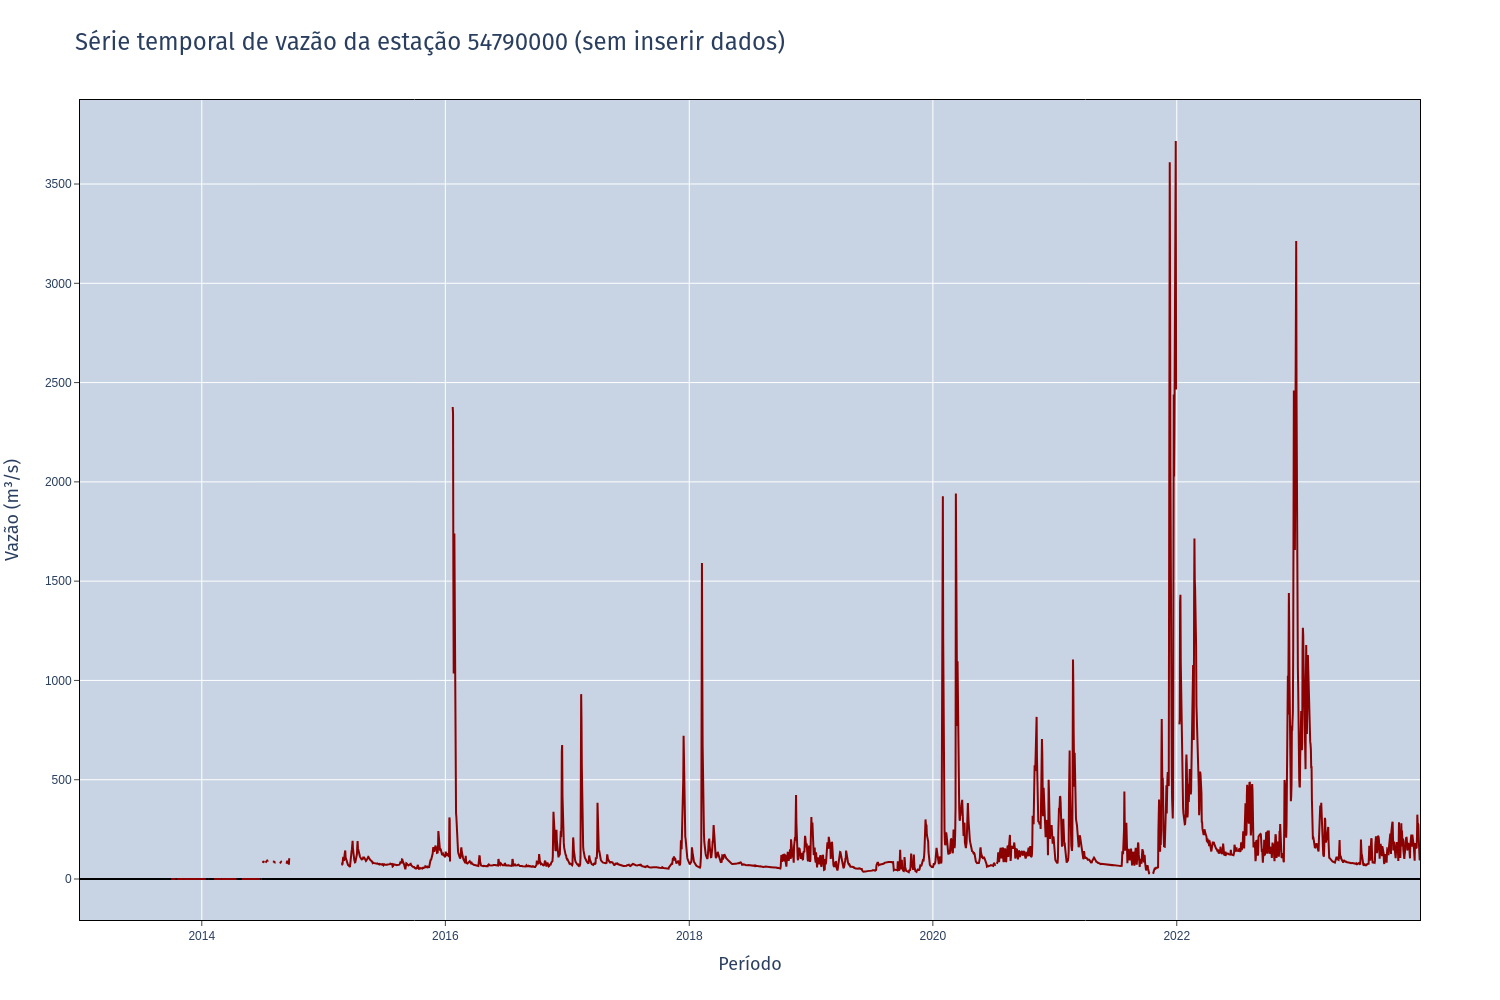
\includegraphics[scale=0.25]{Figuras/jequiti/jequitinhonhaSerieAlvoFaltantes.png}
\caption{Série da estação 54790000 sem dados imputados (fonte: o autor)}
\label{fig:jequitinhonhaSerieAlvoFaltantes}
\end{figure}

Em destaque, a seguir, o trecho da série com mais dados faltantes (figura \ref{fig:jequitinhonhaSerieAlvoFaltantes_2013_2016}). Compreende o período de janeiro de 2013 a janeiro de 2016. Logo após é mostrado como ficou depois de imputar os dados (figura \ref{fig:jequitinhonhaSerieAlvoImputados_2013_2016}). Não ficou exatamente bom este trecho, evidentemente. A imputação colocou vazão zero para vários dias, o que não faz sentido concretamente, pois isso significaria que o rio secou. Ao final da análise, entretanto, estes valores zero não interferiram no resultado, visto que estavam distantes do tempo presente do trabalho. Uma opção seria remover todo trecho anterior ao ano de 2016, mas buscou-se uma uniformidade quanto ao critério de aproveitamento dos dados neste trabalho, visto que havia outros rios a serem analisados e a preocupação de um comportamento que fosse semelhante nos resultados.

\begin{figure}[!h]
\centering
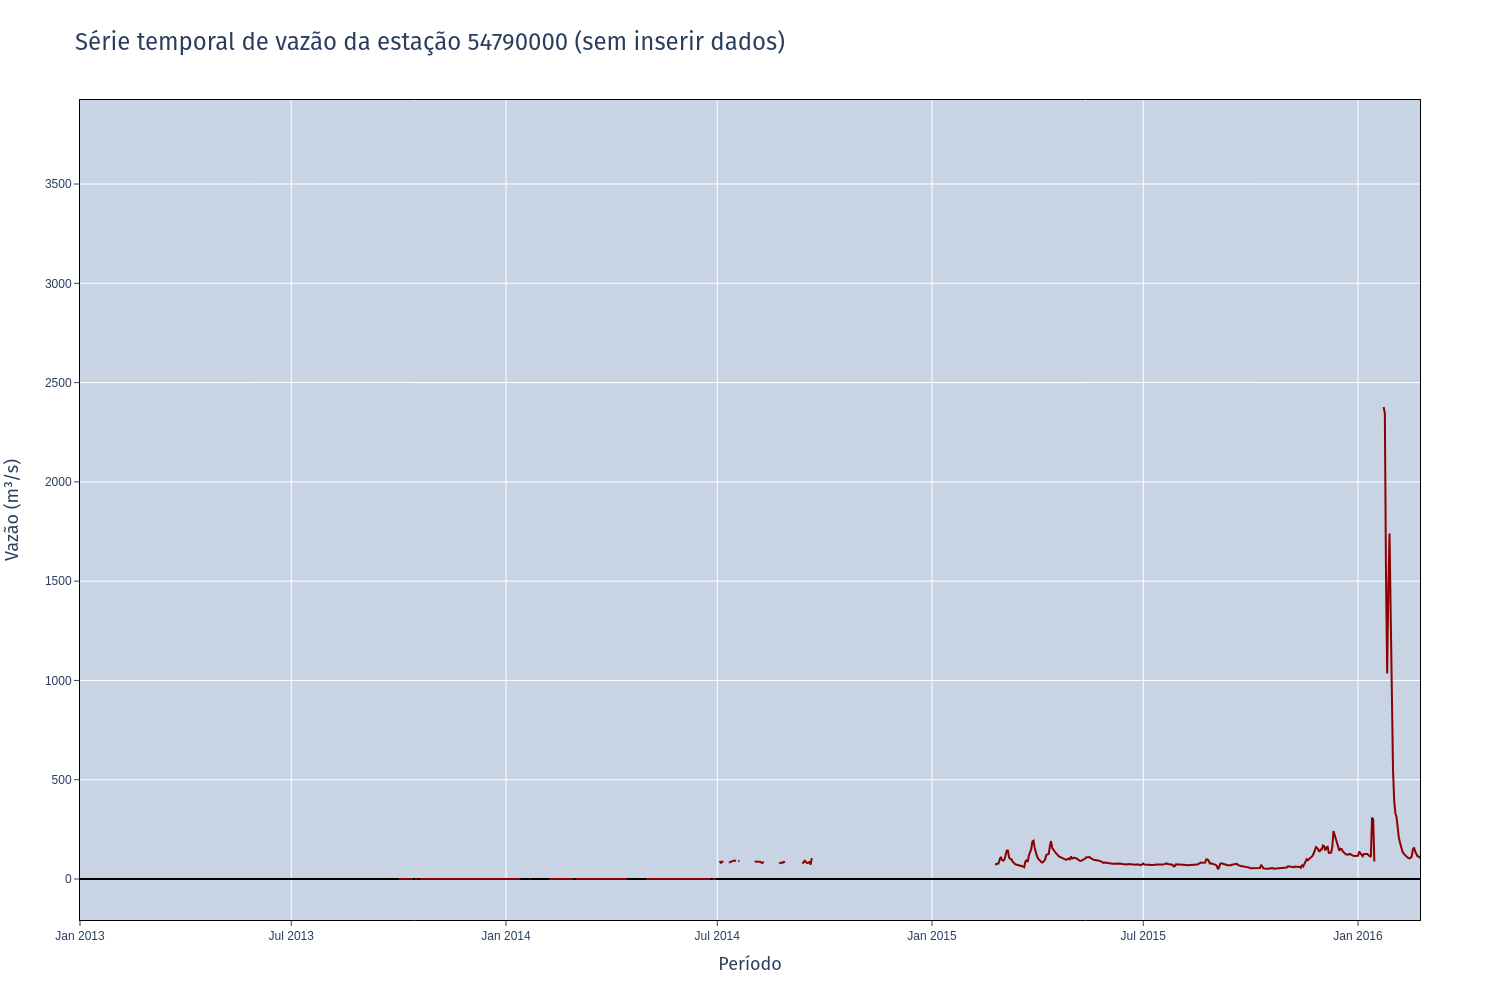
\includegraphics[scale=0.25]{Figuras/jequiti/jequitinhonhaSerieAlvoFaltantes_2013_2016.png}
\caption{Série da estação de vazão 54790000 sem dados imputados de 2013 - 2016 (fonte: o autor)}
\label{fig:jequitinhonhaSerieAlvoFaltantes_2013_2016}
\end{figure}


\begin{figure}[!h]
\centering
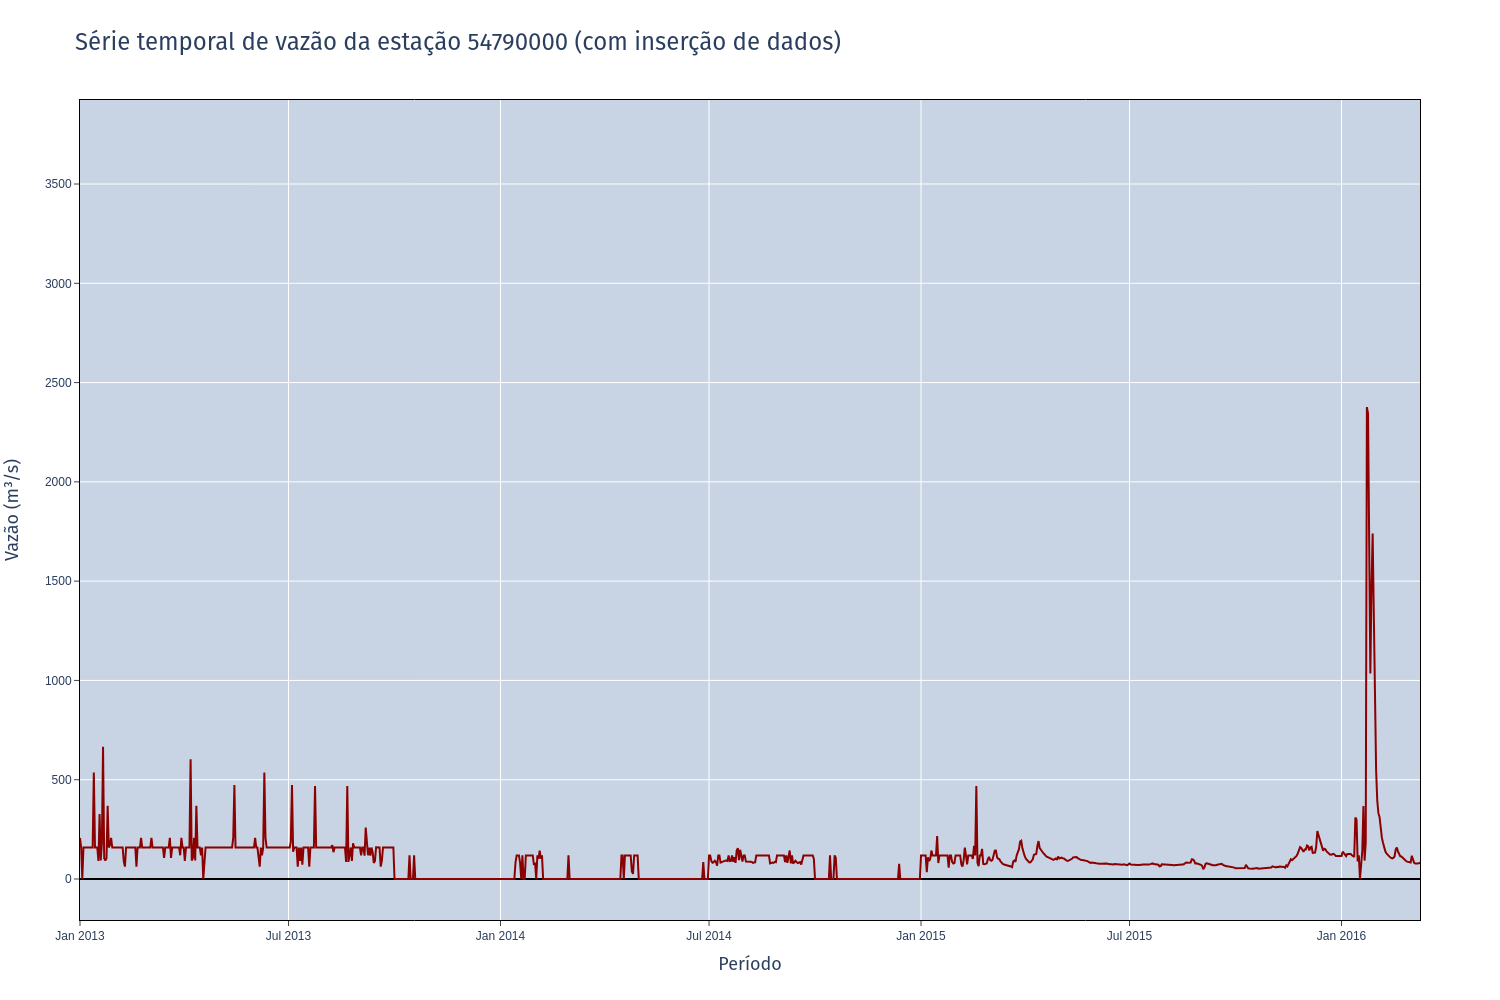
\includegraphics[scale=0.25]{Figuras/jequiti/jequitinhonhaSerieAlvoImputados_2013_2016.png}
\caption{Série da estação de vazão 54790000 com dados imputados de 2013 - 2016 (fonte: o autor)}
\label{fig:jequitinhonhaSerieAlvoImputados_2013_2016}
\end{figure}

Observe também o trecho de dados faltantes mais próximo ao final dos anos analisados, em 2021 e 2022 (figura \ref{fig:jequitinhonhaSerieAlvoFaltantes_2021_2022}). Esta porção da série ficou boa visto que havia informação prévia suficiente, a inserção de dados respeitou coerentemente a sazonalidade (figura \ref{fig:jequitinhonhaSerieAlvoImputados_2021_2022}).

\begin{figure}[!h]
\centering
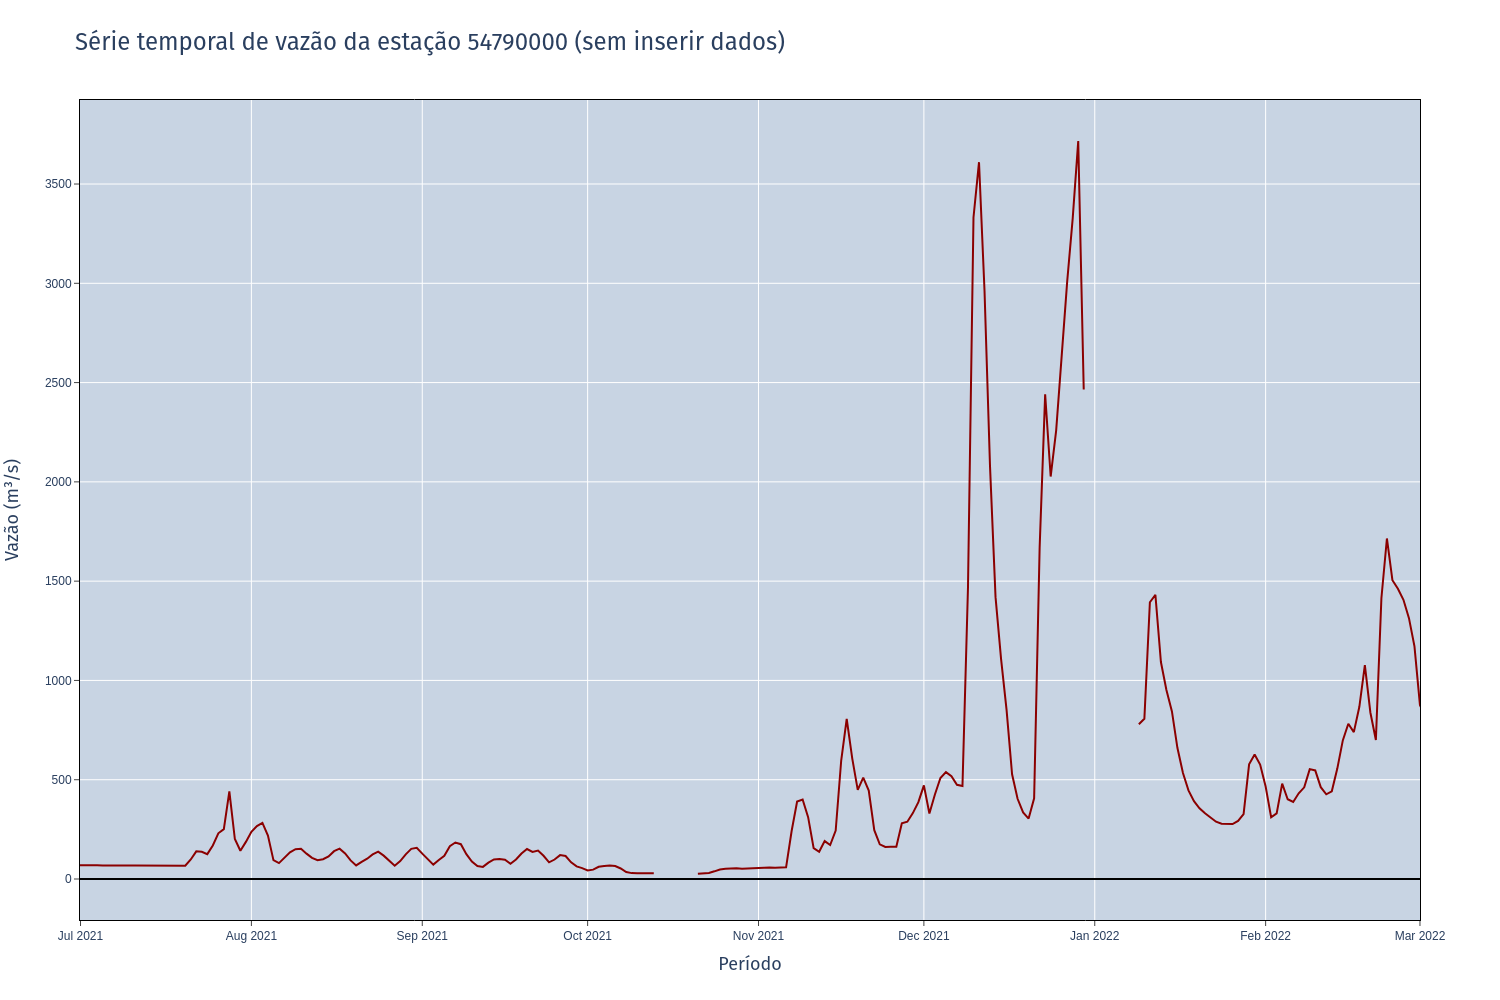
\includegraphics[scale=0.25]{Figuras/jequiti/jequitinhonhaSerieAlvoFaltantes_2021_2022.png}
\caption{Série da estação de vazão 54790000 sem dados imputados 2021/2022 (fonte: o autor)}
\label{fig:jequitinhonhaSerieAlvoFaltantes_2021_2022}
\end{figure}

\begin{figure}[!h]
\centering
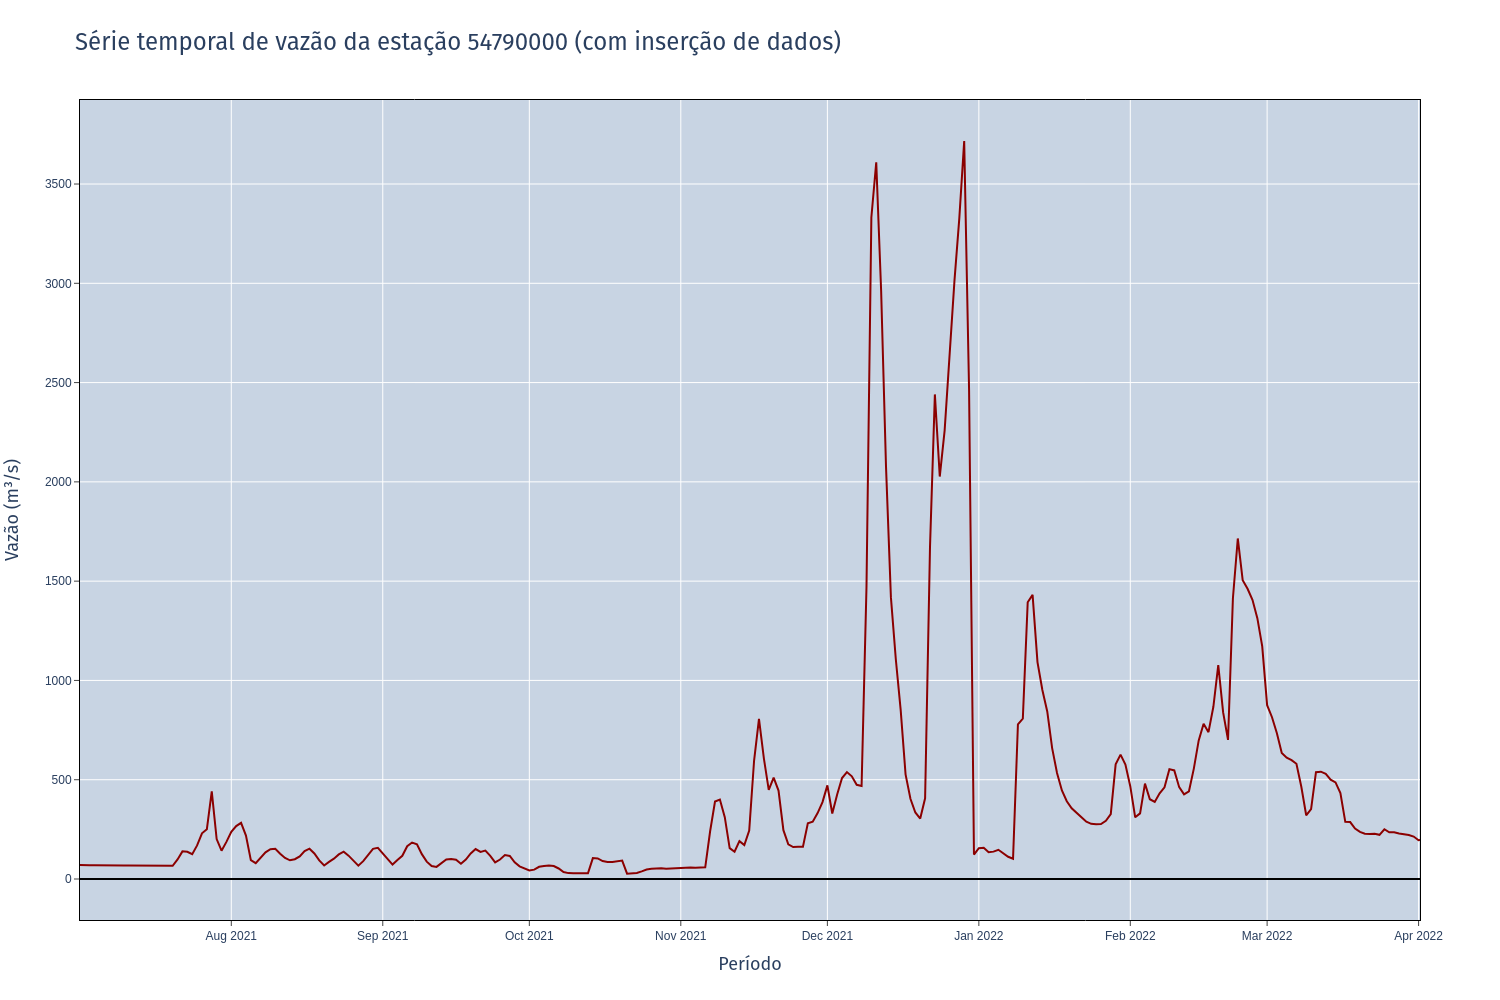
\includegraphics[scale=0.25]{Figuras/jequiti/jequitinhonhaSerieAlvoImputados_2021_2022.png}
\caption{Série da estação de vazão 54790000 com dados imputados 2021/2022 (fonte: o autor)}
\label{fig:jequitinhonhaSerieAlvoImputados_2021_2022}
\end{figure}

\newpage
Por fim, uma visão ampla de como ficou a série temporal após os procedimentos de imputação dos dados. (figura \ref{fig:jequitinhonhaSerieAlvoImputados})

\begin{figure}[!h]
\centering
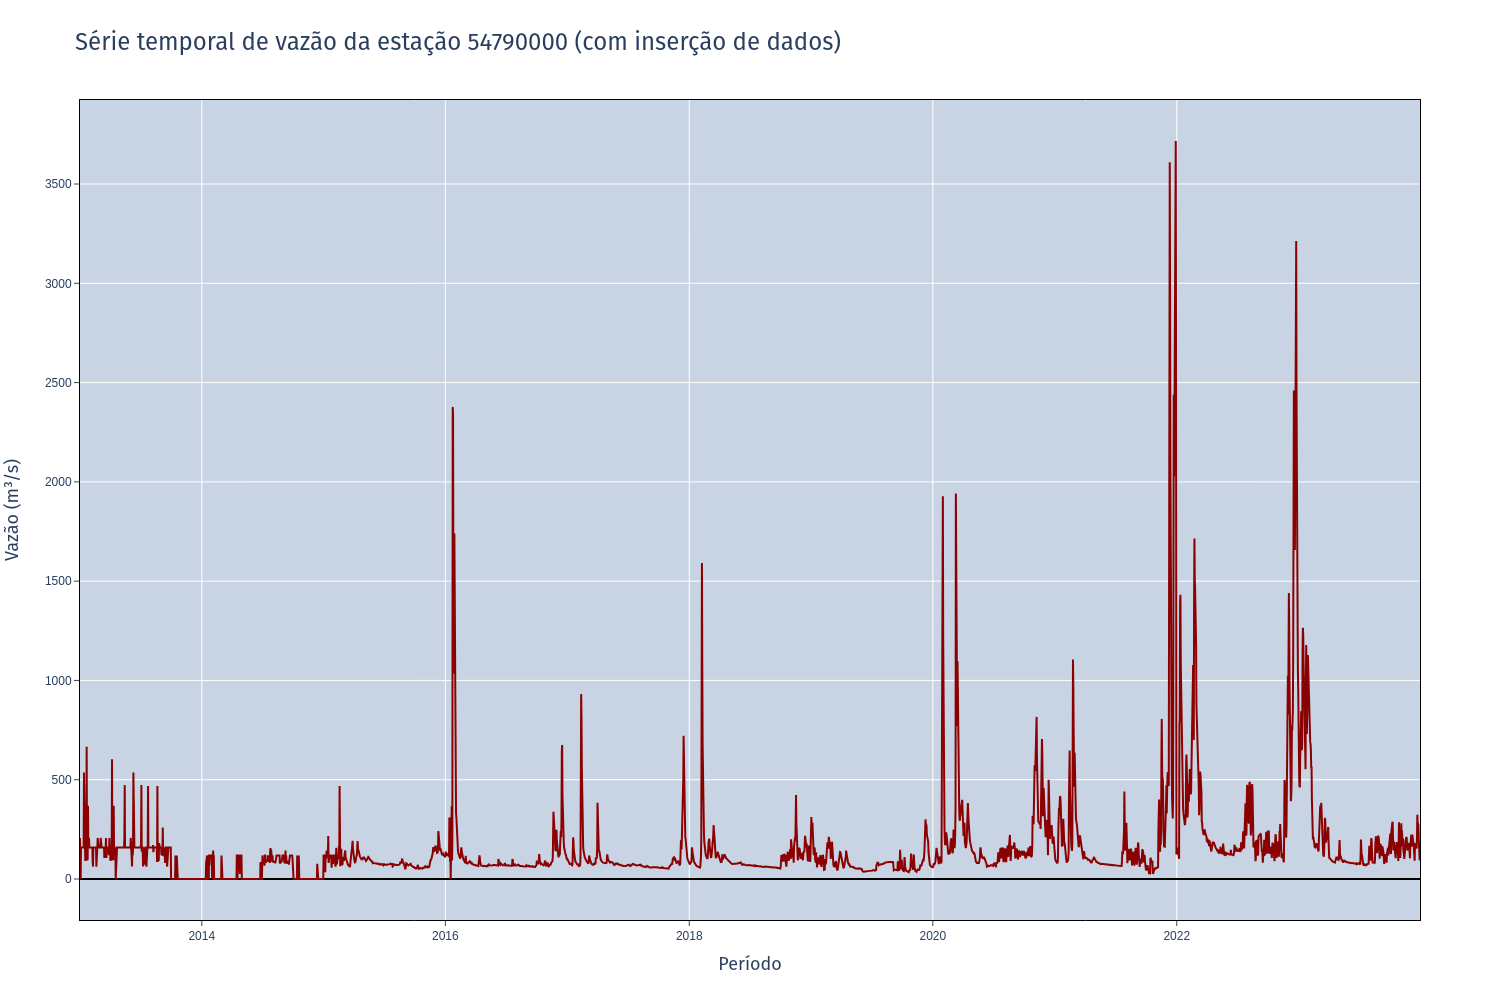
\includegraphics[scale=0.25]{Figuras/jequiti/jequitinhonhaSerieAlvoImputados.png}
\caption{Série da estação 54790000 com dados imputados (fonte: o autor)}
\label{fig:jequitinhonhaSerieAlvoImputados}
\end{figure}

A mesma análise foi realizada para as estações de chuva. Nos dados da estação telemétrica de precipitação de código 54790000 (figura \ref{fig:jequitinhonhaSerieChuvaFaltantes_t_cv_54790000}), faltavam 273 dias de dados (6,79\%). Já a estação convencional de precipitação de código 01640000 estava totalmente preenchida, sem valores nulos. (figura \ref{fig:jequitinhonhaSerieChuva_c_cv_01640000})

\begin{figure}[!h]
\centering
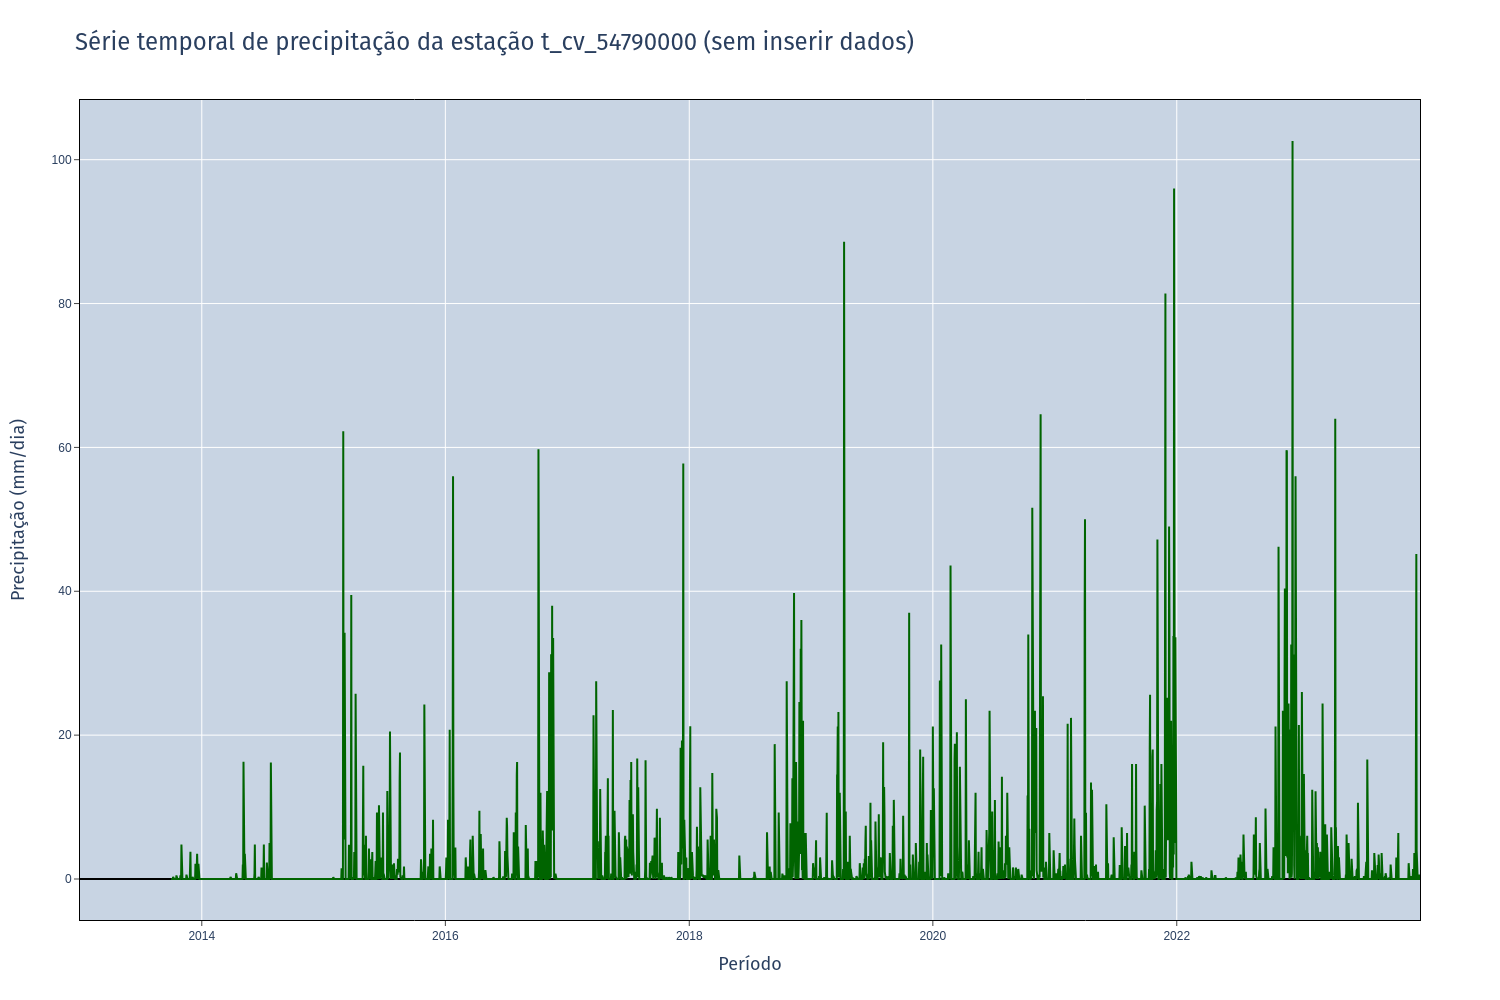
\includegraphics[scale=0.25]{Figuras/jequiti/jequitinhonhaSerieChuvaFaltantes_t_cv_54790000.png}
\caption{Série da estação de precipitação 54790000 sem dados imputados (fonte: o autor)}
\label{fig:jequitinhonhaSerieChuvaFaltantes_t_cv_54790000}
\end{figure}

Destaque para o trecho da série com dados faltantes, no início da série. (figura \ref{fig:jequitinhonhaSerieChuvaFaltantes_t_cv_54790000_2013})

\begin{figure}[!h]
\centering
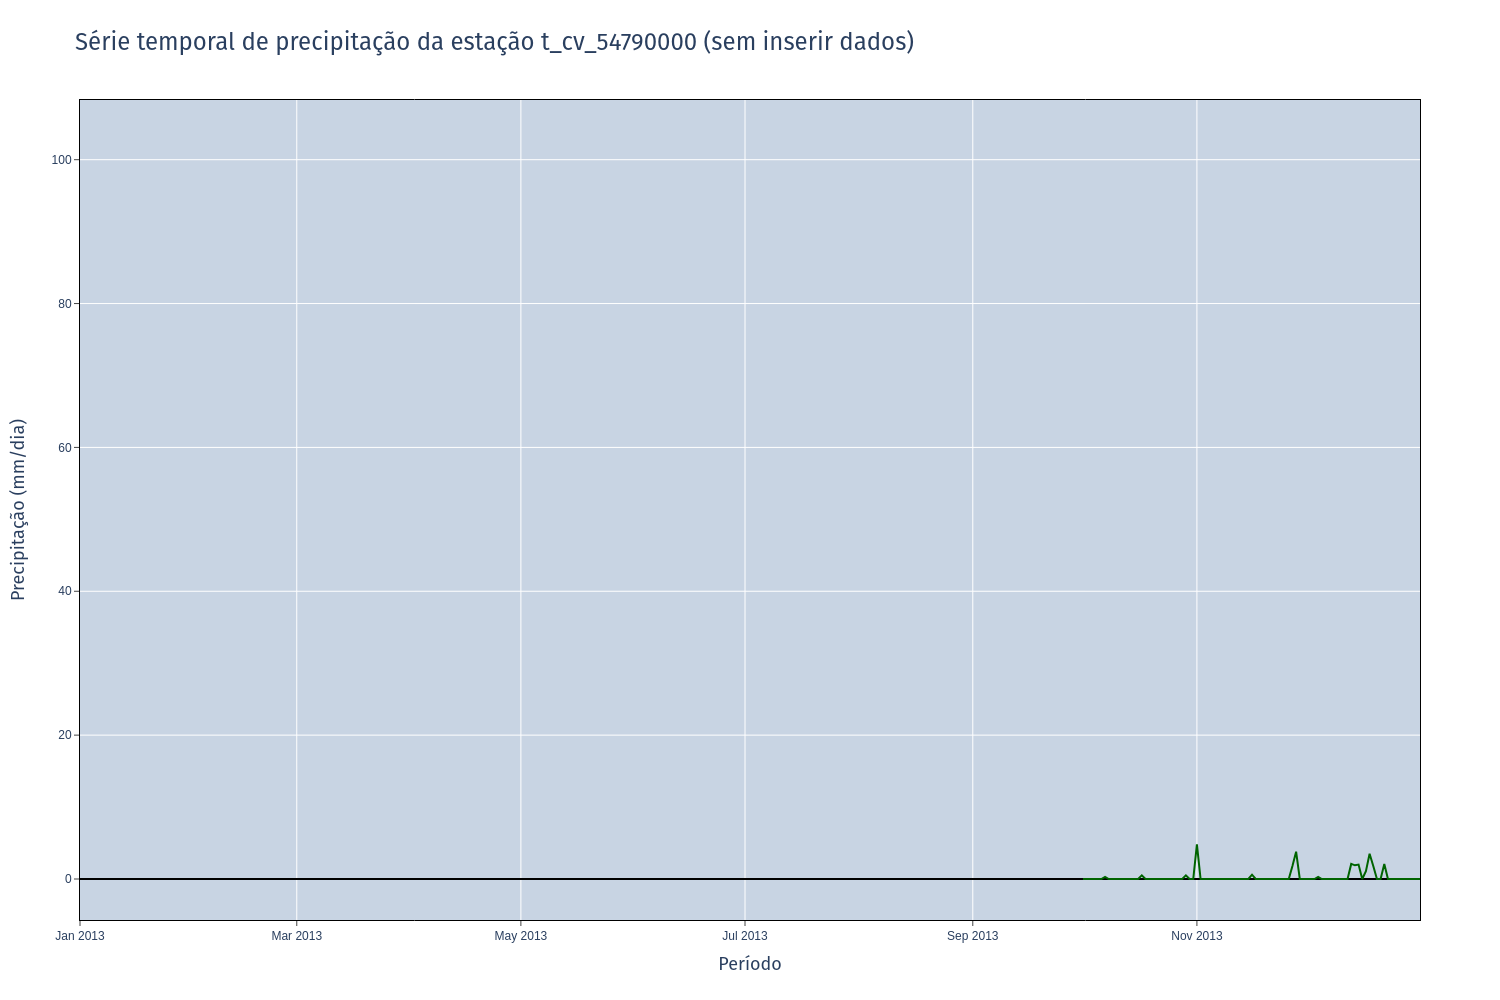
\includegraphics[scale=0.25]{Figuras/jequiti/jequitinhonhaSerieChuvaFaltantes_t_cv_54790000_2013.png}
\caption{Em detalhe, série da estação de precipitação 54790000 sem dados imputados - 2013 (fonte: o autor)}
\label{fig:jequitinhonhaSerieChuvaFaltantes_t_cv_54790000_2013}
\end{figure}

As séries de chuva completas ficaram desta forma. \pagebreak

\begin{figure}[!h]
\centering
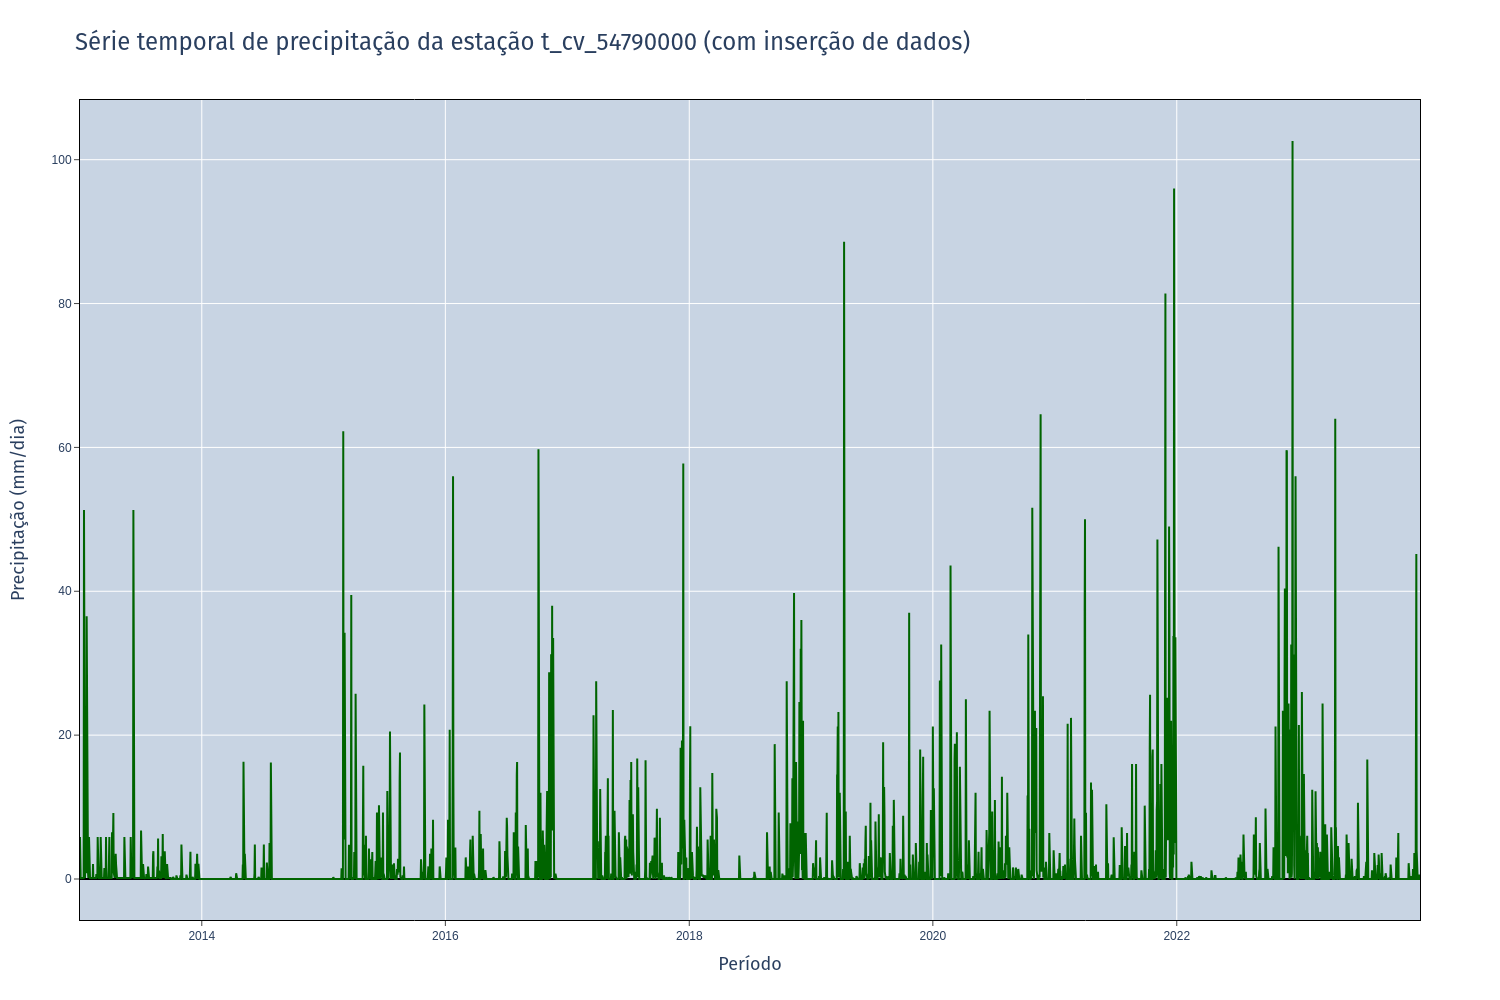
\includegraphics[scale=0.25]{Figuras/jequiti/jequitinhonhaSerieChuvaImputados_t_cv_54790000.png}
\caption{Série da estação de precipitação 54790000 já com dados imputados (fonte: o autor)}
\label{fig:jequitinhonhaSerieChuvaImputados_t_cv_54790000}
\end{figure}

\begin{figure}[!h]
\centering
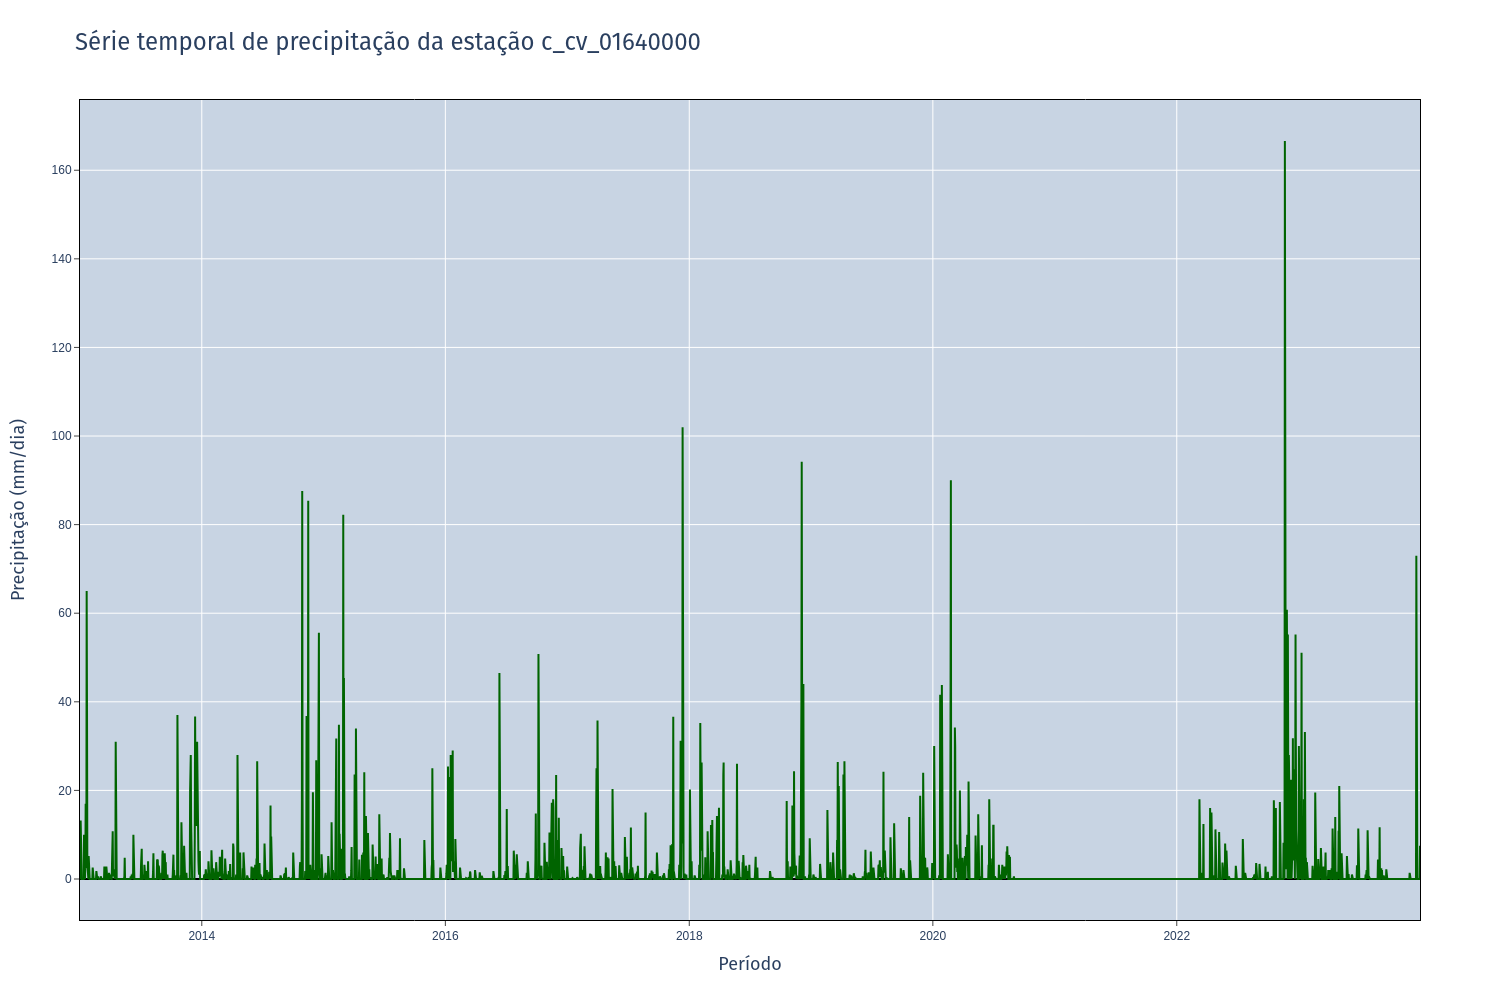
\includegraphics[scale=0.25]{Figuras/jequiti/jequitinhonhaSerieChuva_c_cv_01640000.png}
\caption{Série completa da estação de precipitação 01640000 (fonte: o autor)}
\label{fig:jequitinhonhaSerieChuva_c_cv_01640000}
\end{figure}

\subsection{Rio Doce}

A série de vazão para o rio Doce foi a que apresentou melhor qualidade no que diz respeito aos dados obtidos. Havia falta de apenas 3 dias, dos 4017 dias do período inteiro. Apenas o preenchimento sazonal bastou para completar a série e não foi preciso mais que isso. Cabe destacar a sazonalidade da série. Ficou bastante evidente este comportamento.

\begin{figure}[!h]
\centering
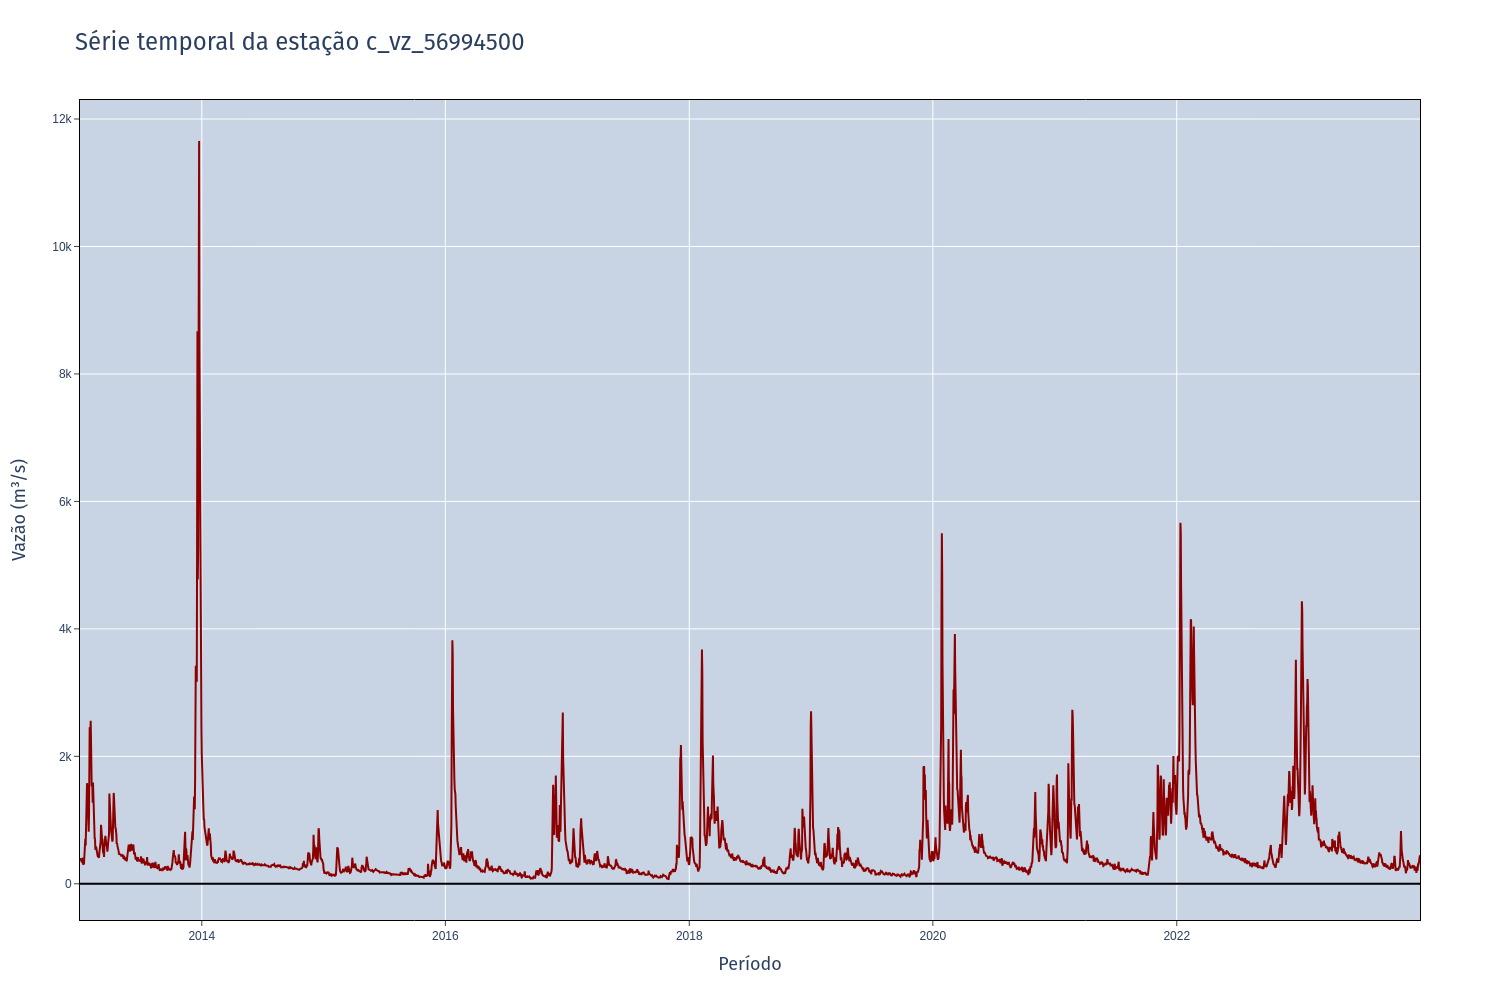
\includegraphics[scale=0.25]{Figuras/rio_doce/rioDoceSerie_c_vz_56994500_completa.png}
\caption{Série completa da estação c\_vz\_56994500 (fonte: o autor)}
\label{fig:rioDoceSerie_c_vz_56994500_completa}
\end{figure}

Se para os dados de vazão no rio Doce a séie foi, digamos, mais comportada, o mesmo não se pode dizer exatamente das estações de chuva. Ao menos, não para duas delas. Estas estações tiveram os dados desconsiderados e foram removidos das análise. Primeiro foi a estação t\_cv\_56990850 que possuía valores discrepantes demais para serem considerados. Valores da ordem de 7000 mm/dia, 8500 mm/dia. (\ref{fig:rioDoceSerie_t_cv_56990850_completa})

A outra estação removida foi a t\_cv\_56994500. Conforme pode ser observado (figura \ref{fig:rioDoceSerie_t_cv_56994500_completa}) nela havia um longo hiato de dados zerados, voltando à normalidade apenas mais recentemente. Como as informações de precipitação que deveria haver para a estação no período do hiato, pode ser retirado de outras estações usadas na modelagem, optou-se por remover esta estação completamente do trabalho.

\begin{figure}[!h]
\centering
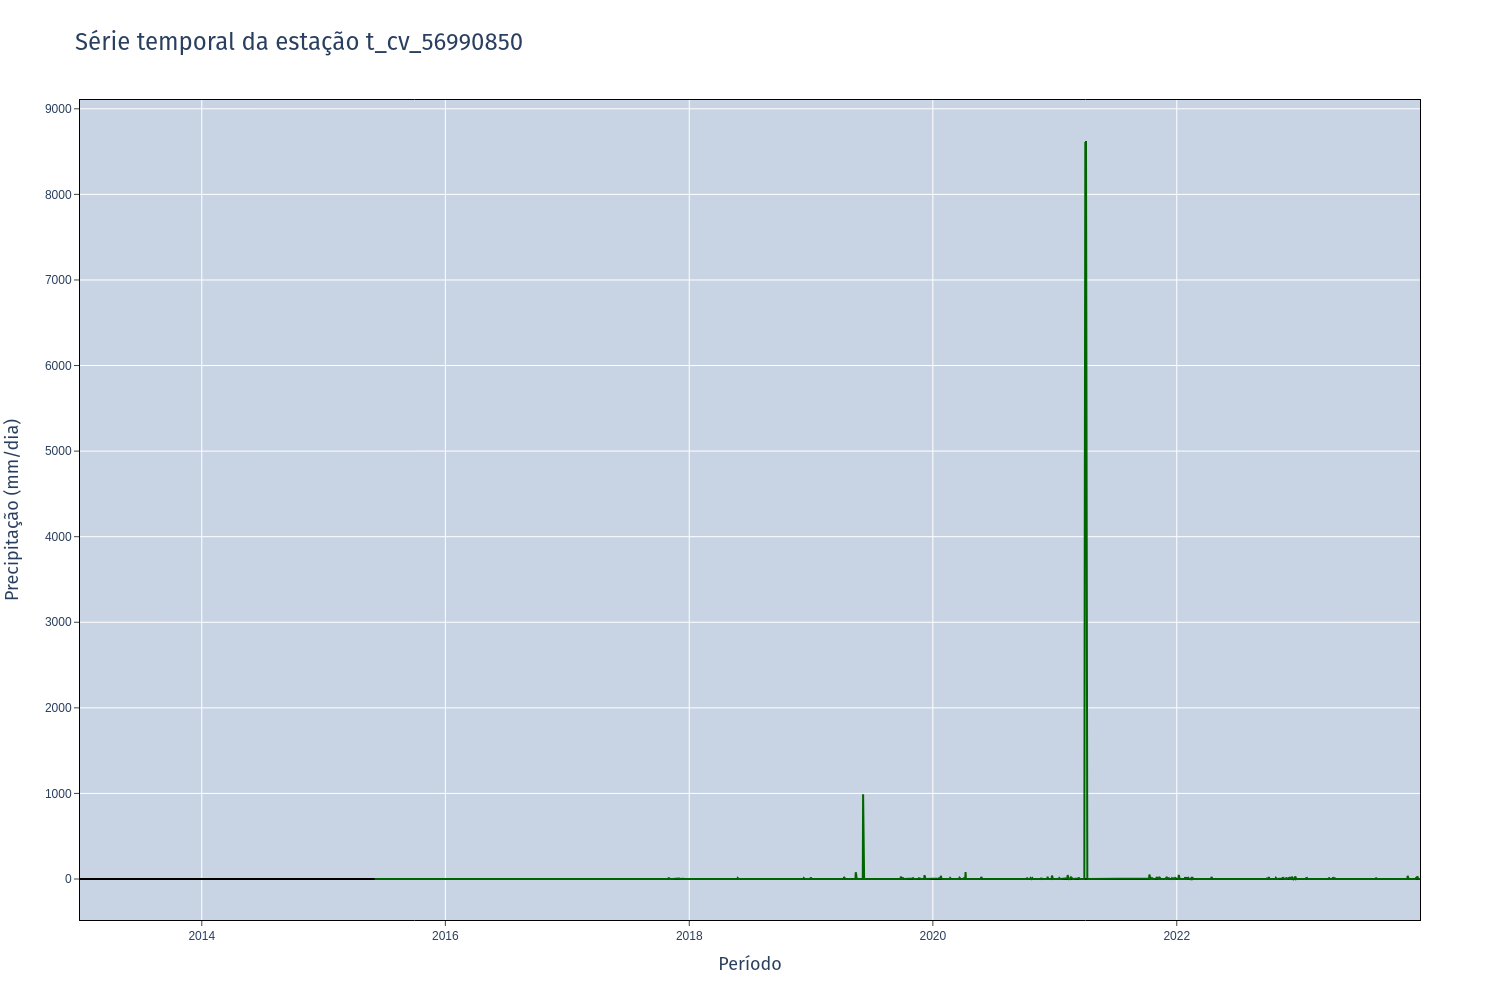
\includegraphics[scale=0.25]{Figuras/rio_doce/rioDoceSerie_t_cv_56990850_completa.png}
\caption{Série completa da estação t\_cv\_56990850 - não utilizada (fonte: o autor)}
\label{fig:rioDoceSerie_t_cv_56990850_completa}
\end{figure}

\begin{figure}[!h]
\centering
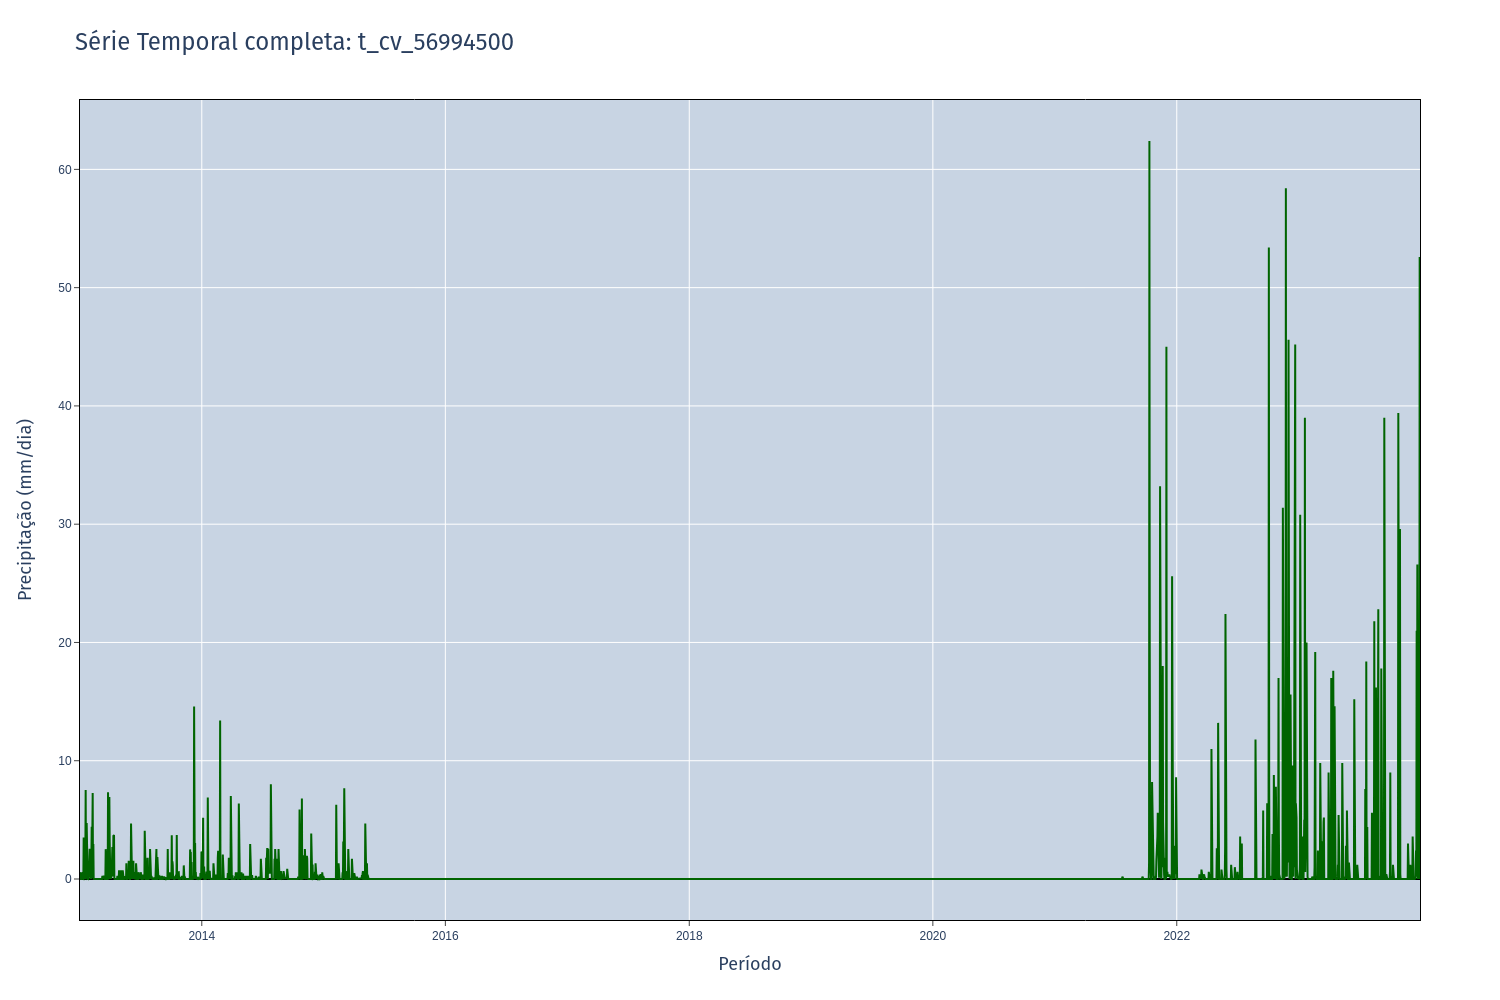
\includegraphics[scale=0.25]{Figuras/rio_doce/rioDoceSerie_t_cv_56994500_completa.png}
\caption{Série completa da estação t\_cv\_56994500 - não utilizada (fonte: o autor)}
\label{fig:rioDoceSerie_t_cv_56994500_completa}
\end{figure}

As estações que, enfim, foram empregadas na modelagem foram as que estão na tabela e adiante, a série temporal de cada uma delas.

\begin{table}[h!]
\centering \small
\caption{Estações de precipitação usadas - final}
\begin{tabular}{|c|c|c|} \hline
\textbf{Estação}&  \textbf{\# dados faltantes}& \textbf{\% dados faltantes} \\ \hline
c\_cv\_01941010 & 153  & 3,81 \\ \hline
c\_cv\_01941004 & 31   & 0,77 \\ \hline
c\_cv\_01941006 & 0    & 0,00 \\ \hline
t\_cv\_56990005 & 1395 & 34,73 \\ \hline
\end{tabular}
\label{tab:estacoes_chuva_usadas_final_rio_doce}
\end{table}

\begin{figure}[!h]
\centering
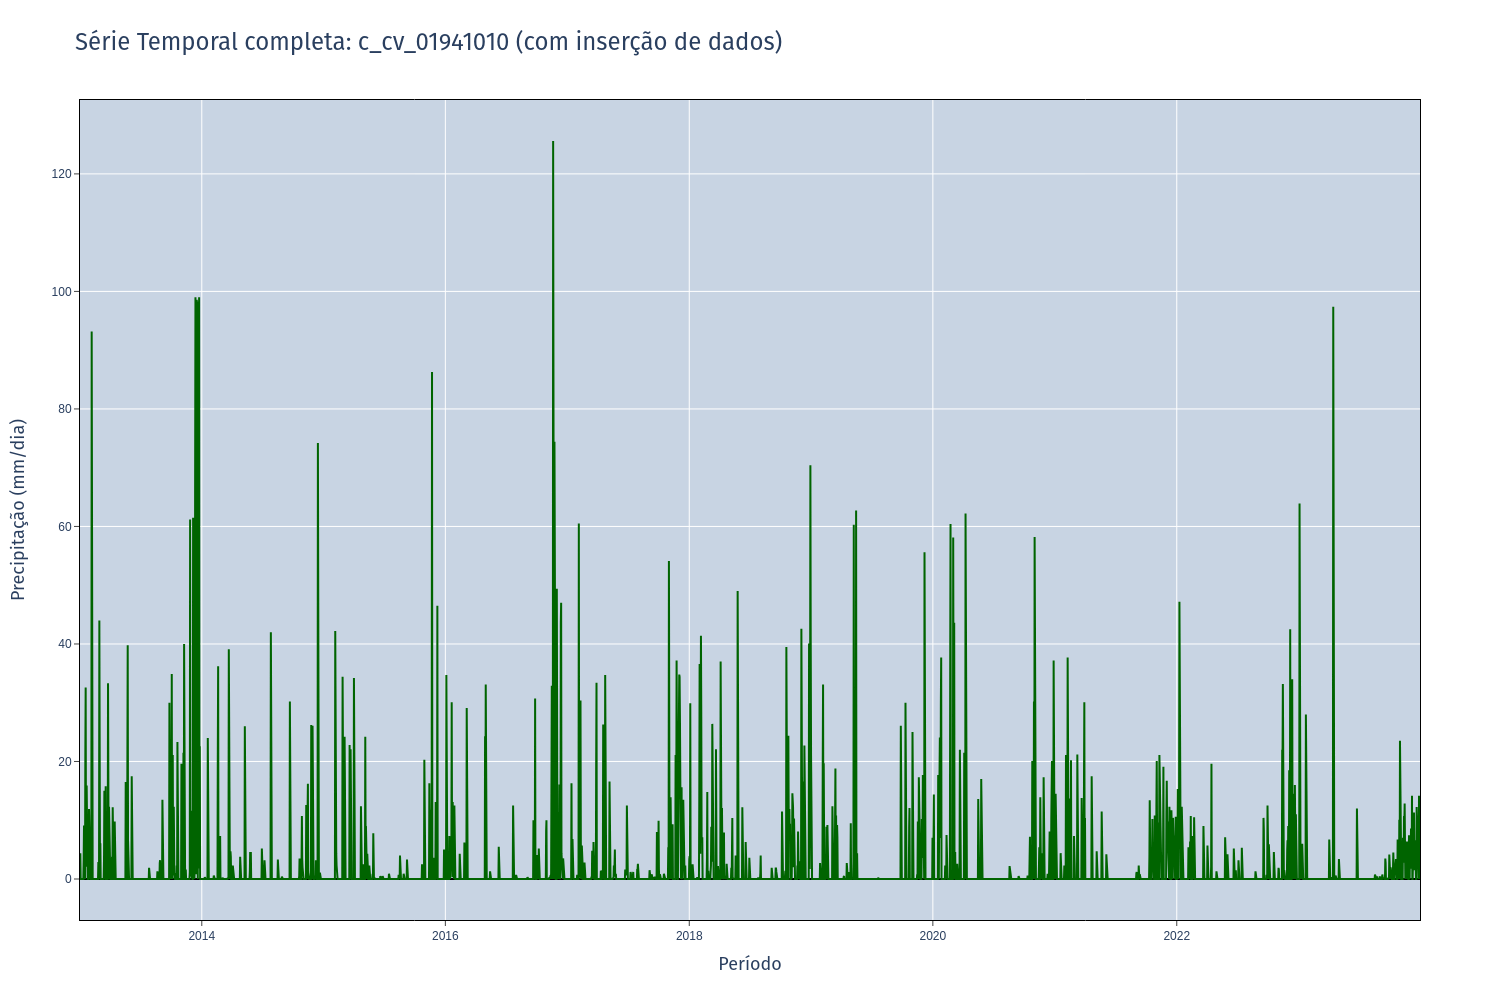
\includegraphics[scale=0.25]{Figuras/rio_doce/rioDoceSerie_c_cv_01941010_completa.png}
\caption{Série completa da estação c\_cv\_01941010 (fonte: o autor)}
\label{fig:rioDoceSerie_c_cv_01941010_completa}
\end{figure}

\begin{figure}[!h]
\centering
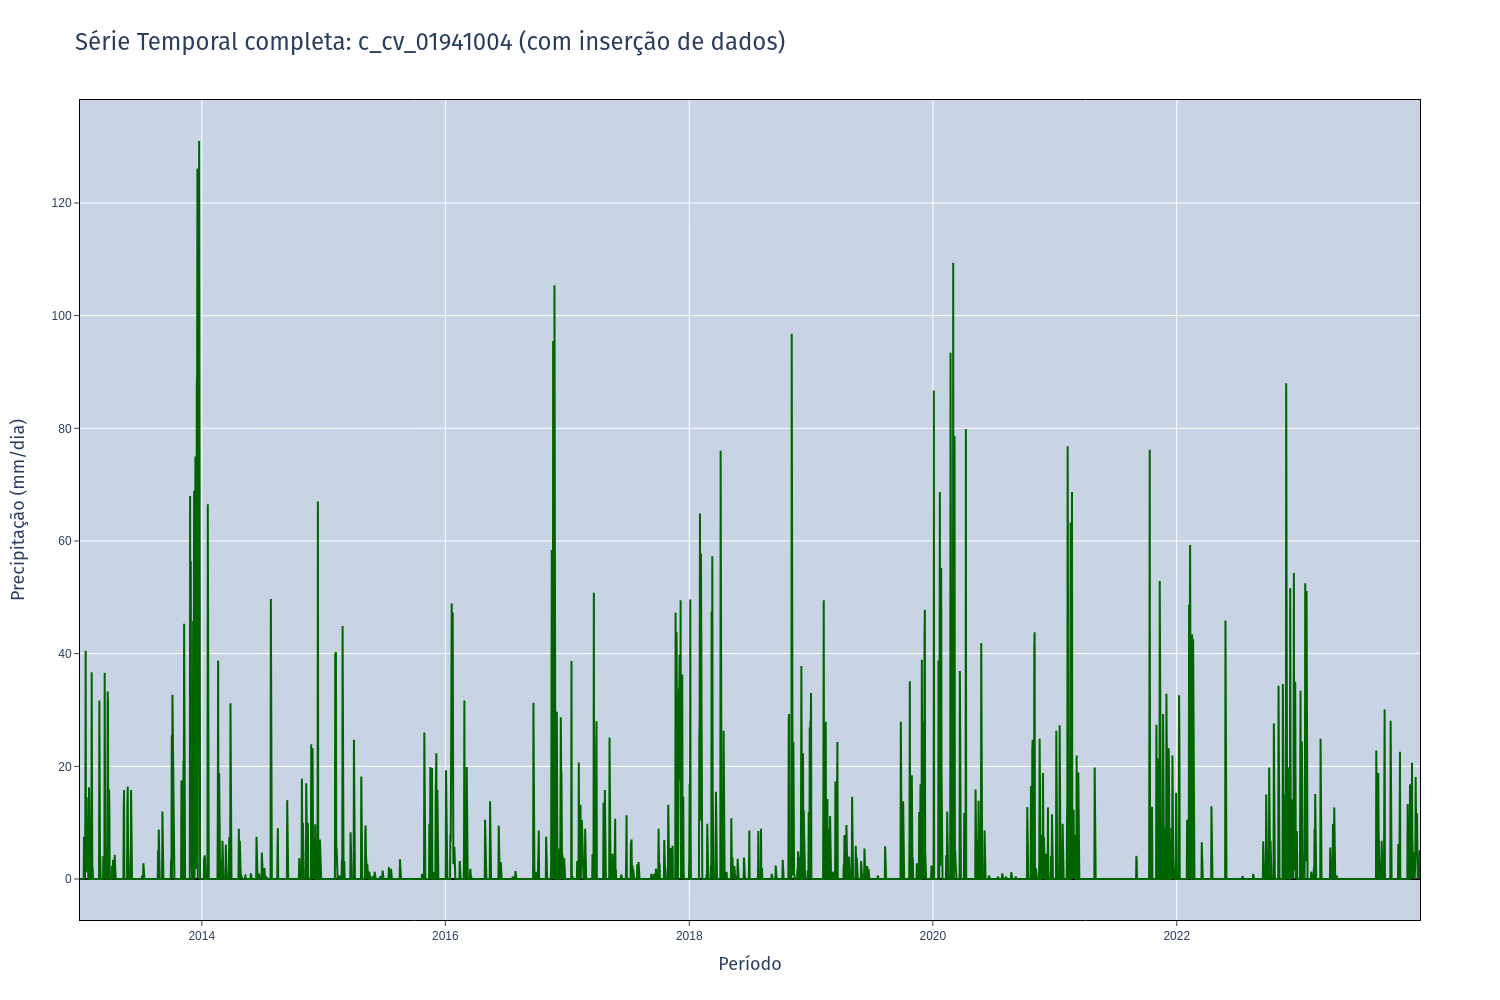
\includegraphics[scale=0.25]{Figuras/rio_doce/rioDoceSerie_c_cv_01941004_completa.png}
\caption{Série completa da estação c\_cv\_01941004 (fonte: o autor)}
\label{fig:rioDoceSerie_c_cv_01941004_completa}
\end{figure}

\begin{figure}[!h]
\centering
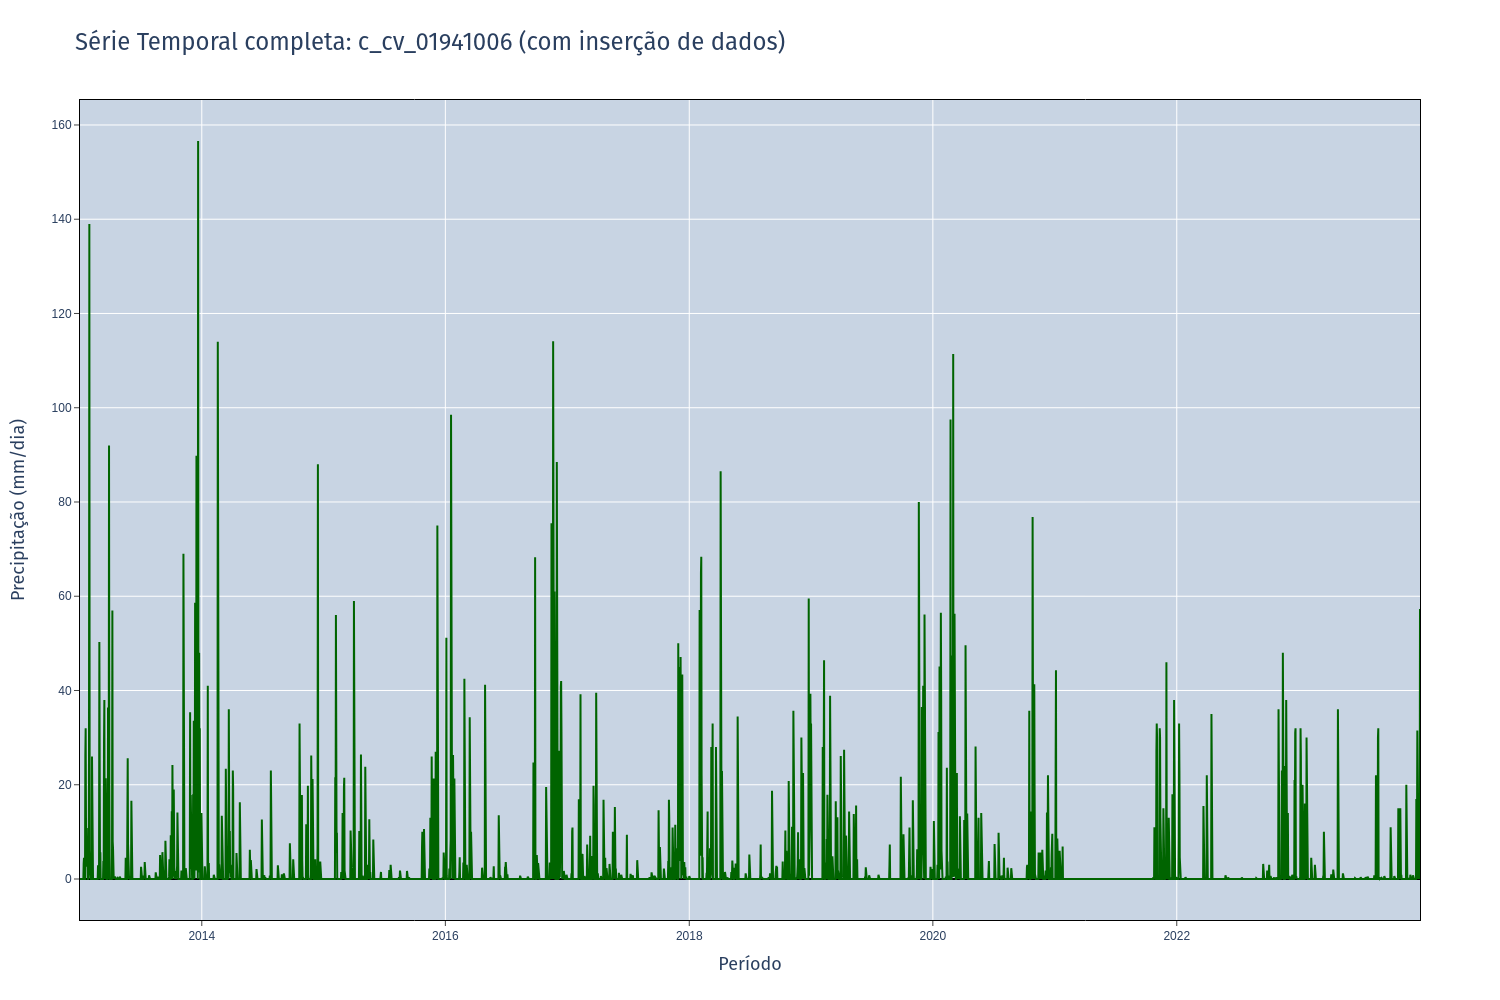
\includegraphics[scale=0.25]{Figuras/rio_doce/rioDoceSerie_c_cv_01941006_completa.png}
\caption{Série completa da estação c\_cv\_01941006 (fonte: o autor)}
\label{fig:rioDoceSerie_c_cv_01941006_completa}
\end{figure}

\begin{figure}[!h]
\centering
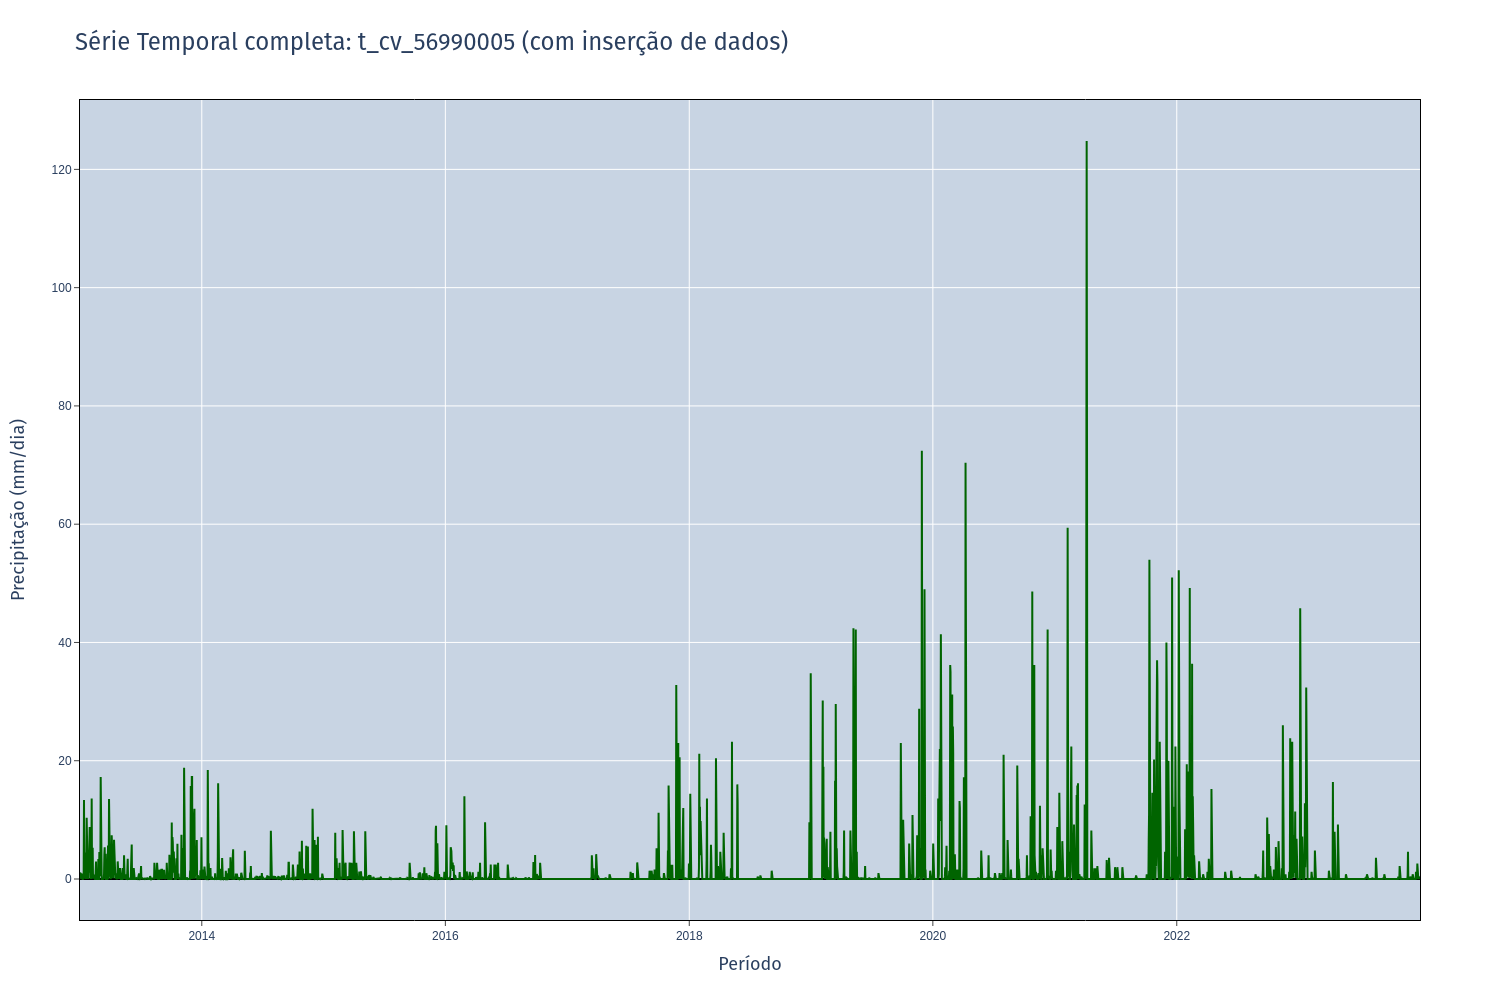
\includegraphics[scale=0.25]{Figuras/rio_doce/rioDoceSerie_t_cv_56990005_completa.png}
\caption{Série completa da estação t\_cv\_56990005 (fonte: o autor)}
\label{fig:rioDoceSerie_t_cv_56990005_completa}
\end{figure}

\subsection{Rio Grande}

O rio Grande foi um desafio à parte em todo trabalho. A dificuldade começou quando não foi encontrada nenhuma estação com dados para o período analisado dentro do estado de Minas Gerais, como mencionado anteriormente. Foi preciso buscar o mais próximo possível do limite da divisa com Minas, já no estado de São Paulo, no município de Ilha Solteira. E os desafios não se encerraram aí.

A série de vazão da estação analisada não possuía dados em todo período de 11 anos analisados e estava incompleta.(figura \ref{fig:rioGrandeSerieAlvoFaltantes}) Os dados mais antigos datavam do ano 2020. Porém, como salientado anteriormente, por definição do escopo do trabalho, realizou o preenchimento dos dados faltantes, aplicando o mesmo protocolo de respeito à sazonalidade dos dados.

\begin{figure}[!h]
\centering
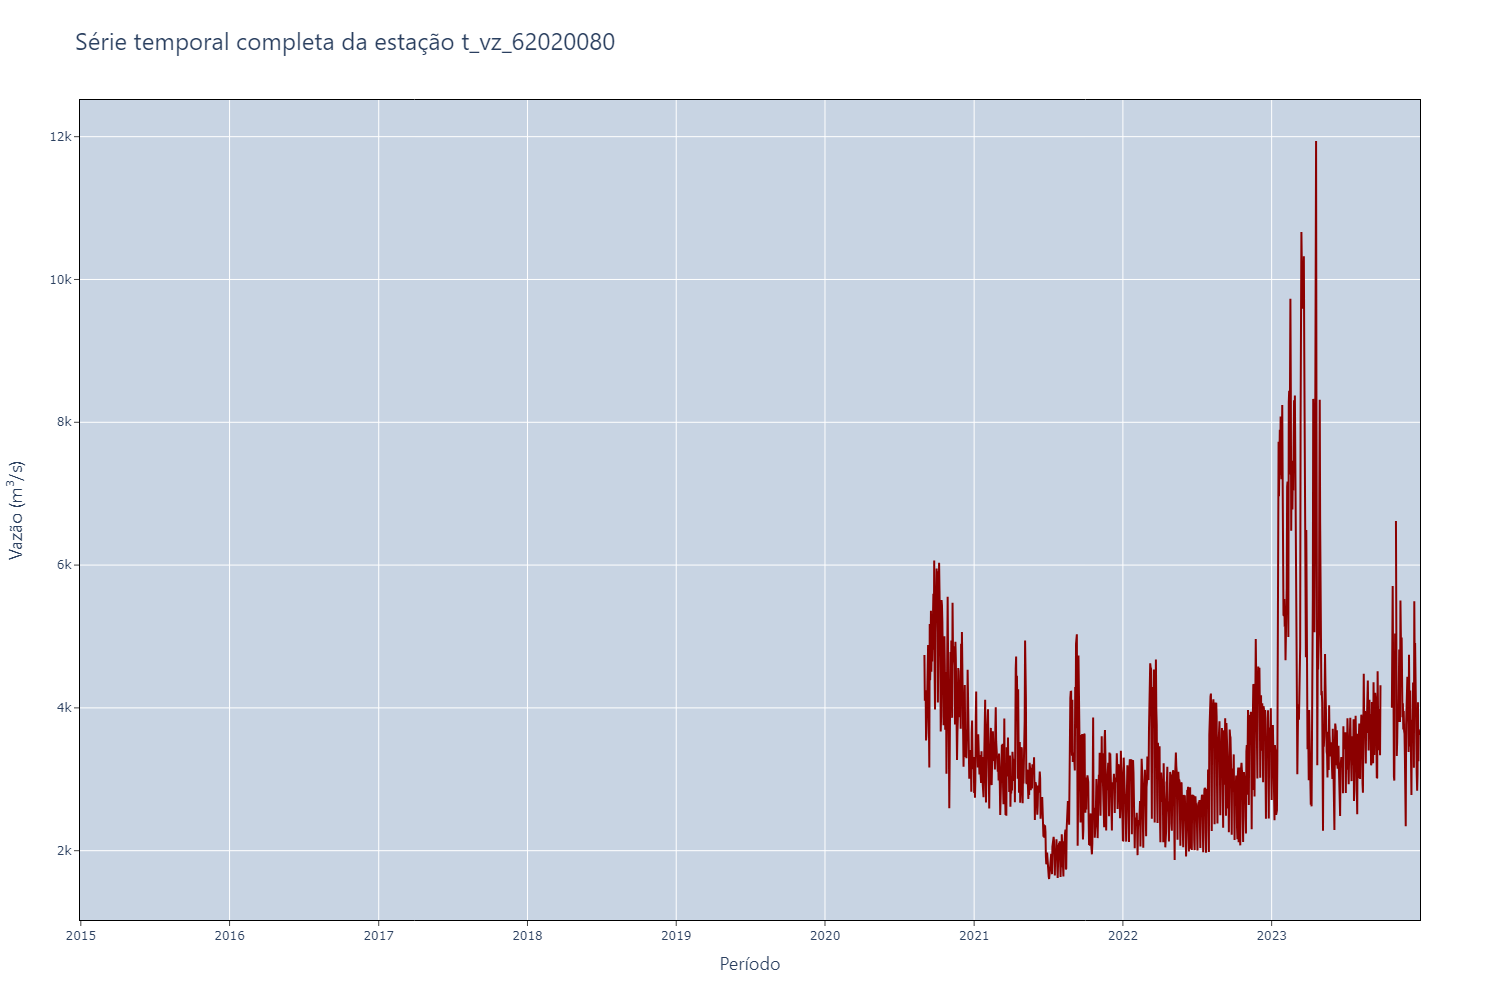
\includegraphics[scale=0.25]{Figuras/rio_grande/rioGrandeSerieAlvoFaltantes.png}
\caption{Série completa da estação t\_vz\_62020080 (fonte: o autor)}
\label{fig:rioGrandeSerieAlvoFaltantes}
\end{figure}

O caráter ruidoso da série, infelizmente, se manteve após a aplicação do protocolo para preenchimento dos dados nulos, como pode ser visto na imagem final gerada. (figura \ref{fig:rioGrandeSerieAlvoImputados}) Esta série contava com 2099 dias faltantes, perfazendo cerca de 64\% de dados nulos. Outro número importante para essa estação é que não foram 4017 registros empregados para o trabalho. O mais distante que havia de informação começava em 2015, de modo que o total de registros para o rio Grande, excepcionalemnte, foi de 3289 registros diários.

\begin{figure}[!h]
\centering
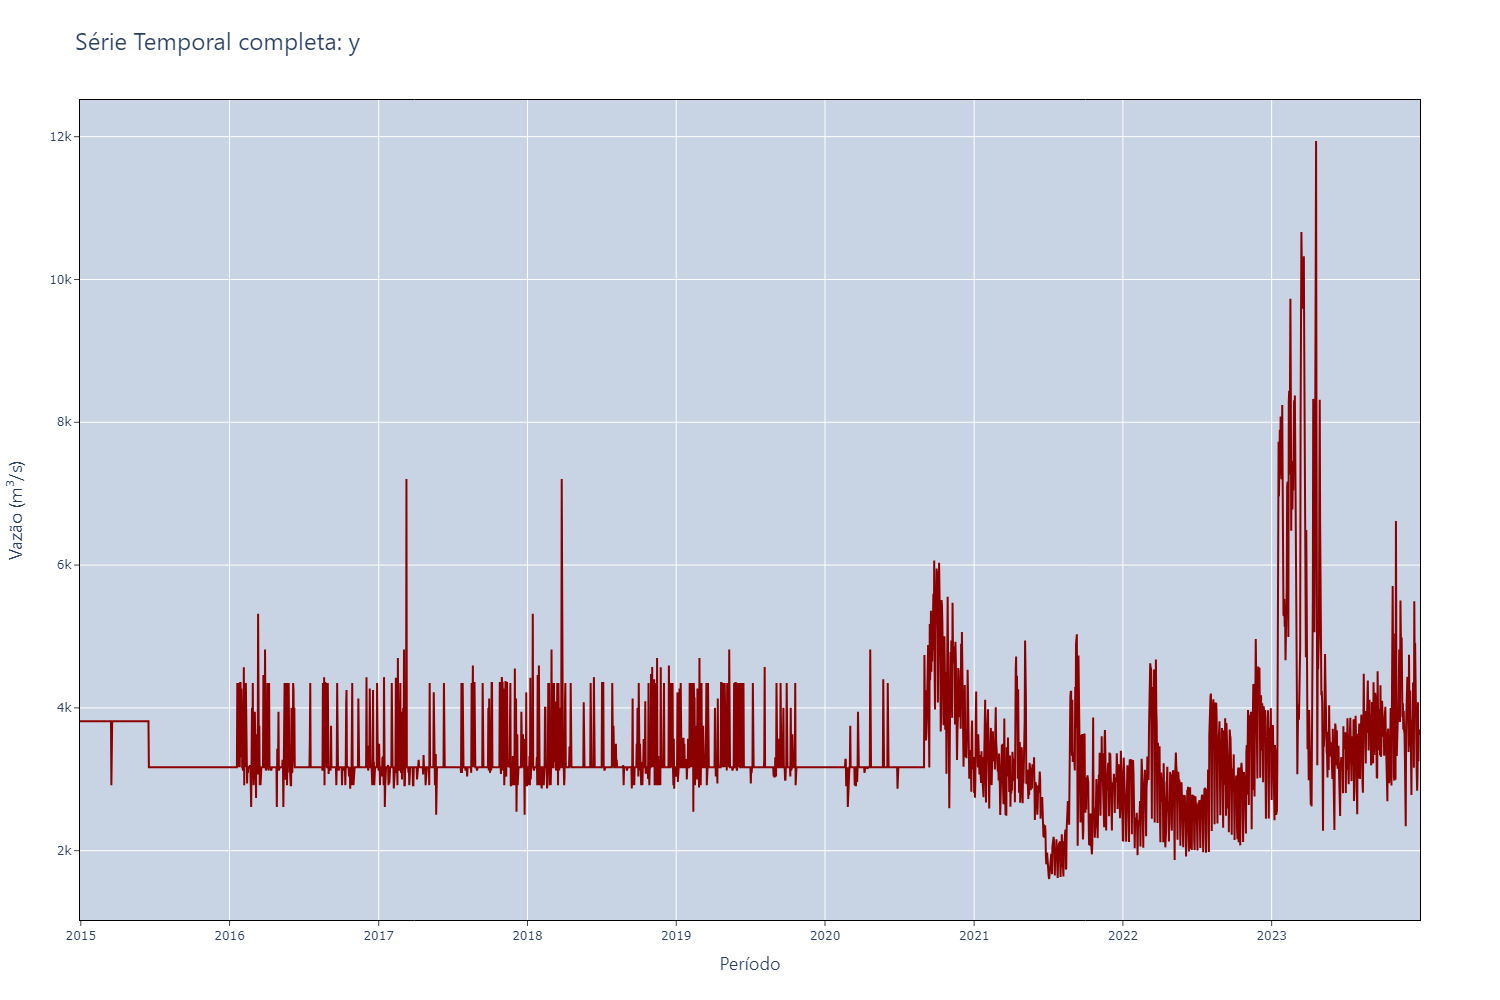
\includegraphics[scale=0.25]{Figuras/rio_grande/rioGrandeSerieAlvoImputados.png}
\caption{Série completa da estação t\_vz\_62020080 (fonte: o autor)}
\label{fig:rioGrandeSerieAlvoImputados}
\end{figure}

A estação de precipitação utilizada, única neste caso, foi a estação t\_cv\_61998080, pois foi a única que apresentou dados. Curiosamente, a outra estação de precipitação apresentou dados para o período analisado, contudo, apenas zeros compunham essa base. Desta forma, a estação t\_cv\_62020080 foi completamente removida do trabalho.

Para a estação t\_cv\_61998080 foi preciso poucos dados a serem preenchidos pois a contagem foi de apenas 169 registros faltando, o que representava 5,14\% do total de dados. (figura \ref{fig:rioGrandeSerieImputado_t_cv_61998080}) Uma série com boa quantidade de dados, de fato, e que puderam contribuir com as análises.

\begin{figure}[!h]
\centering
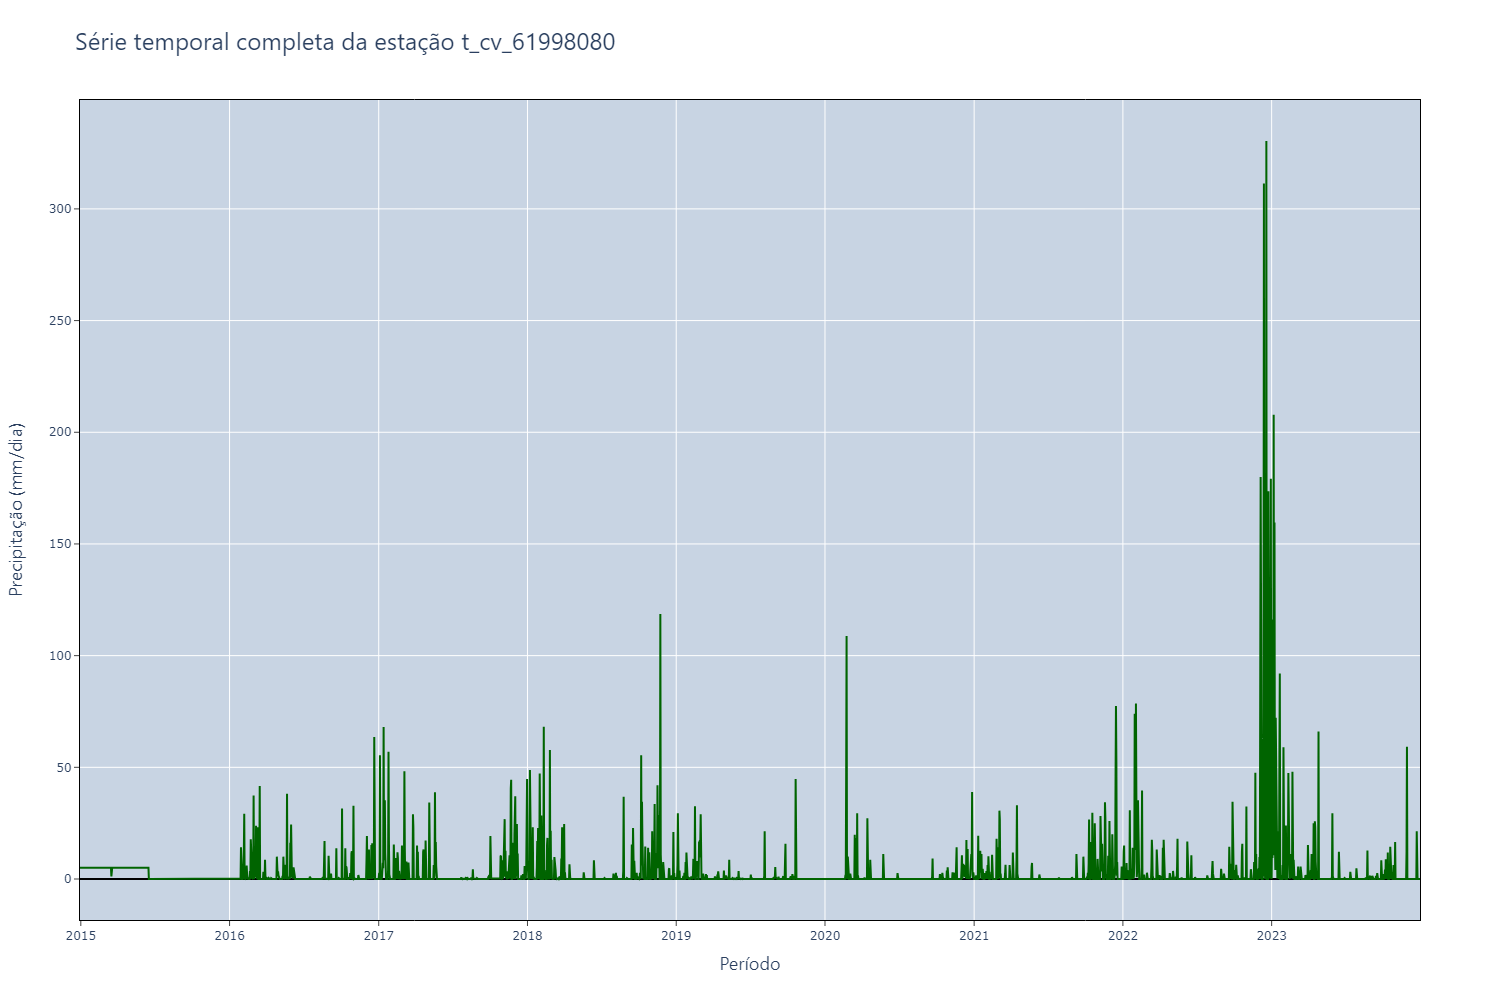
\includegraphics[scale=0.25]{Figuras/rio_grande/rioGrandeSerieImputado_t_cv_61998080.png}
\caption{Série completa da estação t\_cv\_61998080 (fonte: o autor)}
\label{fig:rioGrandeSerieImputado_t_cv_61998080}
\end{figure}

Note que o trecho de dados faltantes está no início da série, no ano de 2015.


%\section{Modelos de Aprendizado de Máquina}
%Apresentar os modelos de ML utilizados (SeasonalNaive, LinearRegression, CatBoost e LightGBM) e justificativas.
%
%\section{Variáveis Utilizadas}
%Listar e explicar as variáveis contínuas e categóricas utilizadas nos modelos.
%
%\section{Treinamento e Validação dos Modelos}
%Detalhar os procedimentos de treinamento e validação dos modelos.
%
%\section{Modelo Proposto}
%Detalhar os procedimentos de treinamento e validação dos modelos.
%\todo[inline]{incluir um workflow que servirá de resumo gráfico}
%
%\section{Métricas de Avaliação}
%Listar as métricas usadas para avaliar o desempenho dos modelos (MAPE, RMSE, PBias* e KGE não-paramétrico**).
%(*: PBias ajuda a ver se o modelo está subestimando as previsões ou superestimando)
%(**: KGEnp (não paramétrico) é uma métrica comum e muito consagrada na hidrologia. Ela tem resiliência a outliers ao avaliar a qualidade do modelo)